\section{Test af System}

\subsection{Hvilke tests}
\begin{frame}{Test}
\framesubtitle{Introduktion}
	
	\begin{itemize}
	\item Intern evaluering
	\item	To bruger test sessions med potentielle brugere, hvor to personer deltog begge gange
		\begin{itemize}
			\item Finde fejl og problemer ved designet
			\item Midtvejs undersøgelse, så problemerne kan løses i kommende sprints.
				\begin{itemize}
					\item 6 test sessions
					\item ca 25 minutter pr session
				\end{itemize}
			\item Afsluttende tests for at finde stadige problemer, samt at modtage holdninger til fremtidig brug af hjemmesiden.
				\begin{itemize}
					\item 7 test sessions
					\item ca 25 minutter pr session
				\end{itemize}
		\end{itemize}
	\item 	Black-Box Unit Tests
	
	\end{itemize}
	
\end{frame}

\begin{frame}{Brugertests}
	\subsection{Udførelse}
	\framesubtitle{Udførelse}
	
	\begin{itemize}
		\item Opgaver 
		\item Tænke højt
		\item Notater
		\item Video	
	\end{itemize}
	
	Evaluering af testene:
	\begin{itemize}
		\item Kosmetisk
		\item Seriøs
		\item Kritisk
	\end{itemize}
	
\end{frame}
	
\begin{frame}{Resultater}
\subsection{Resultater}
\framesubtitle{Indstillinger}
	\subsubsection{Indstillinger}
	
	\begin{minipage}[0.3\textheight]{\textwidth}
	\begin{columns}[T]
	\begin{column}{0.5\textwidth}
	 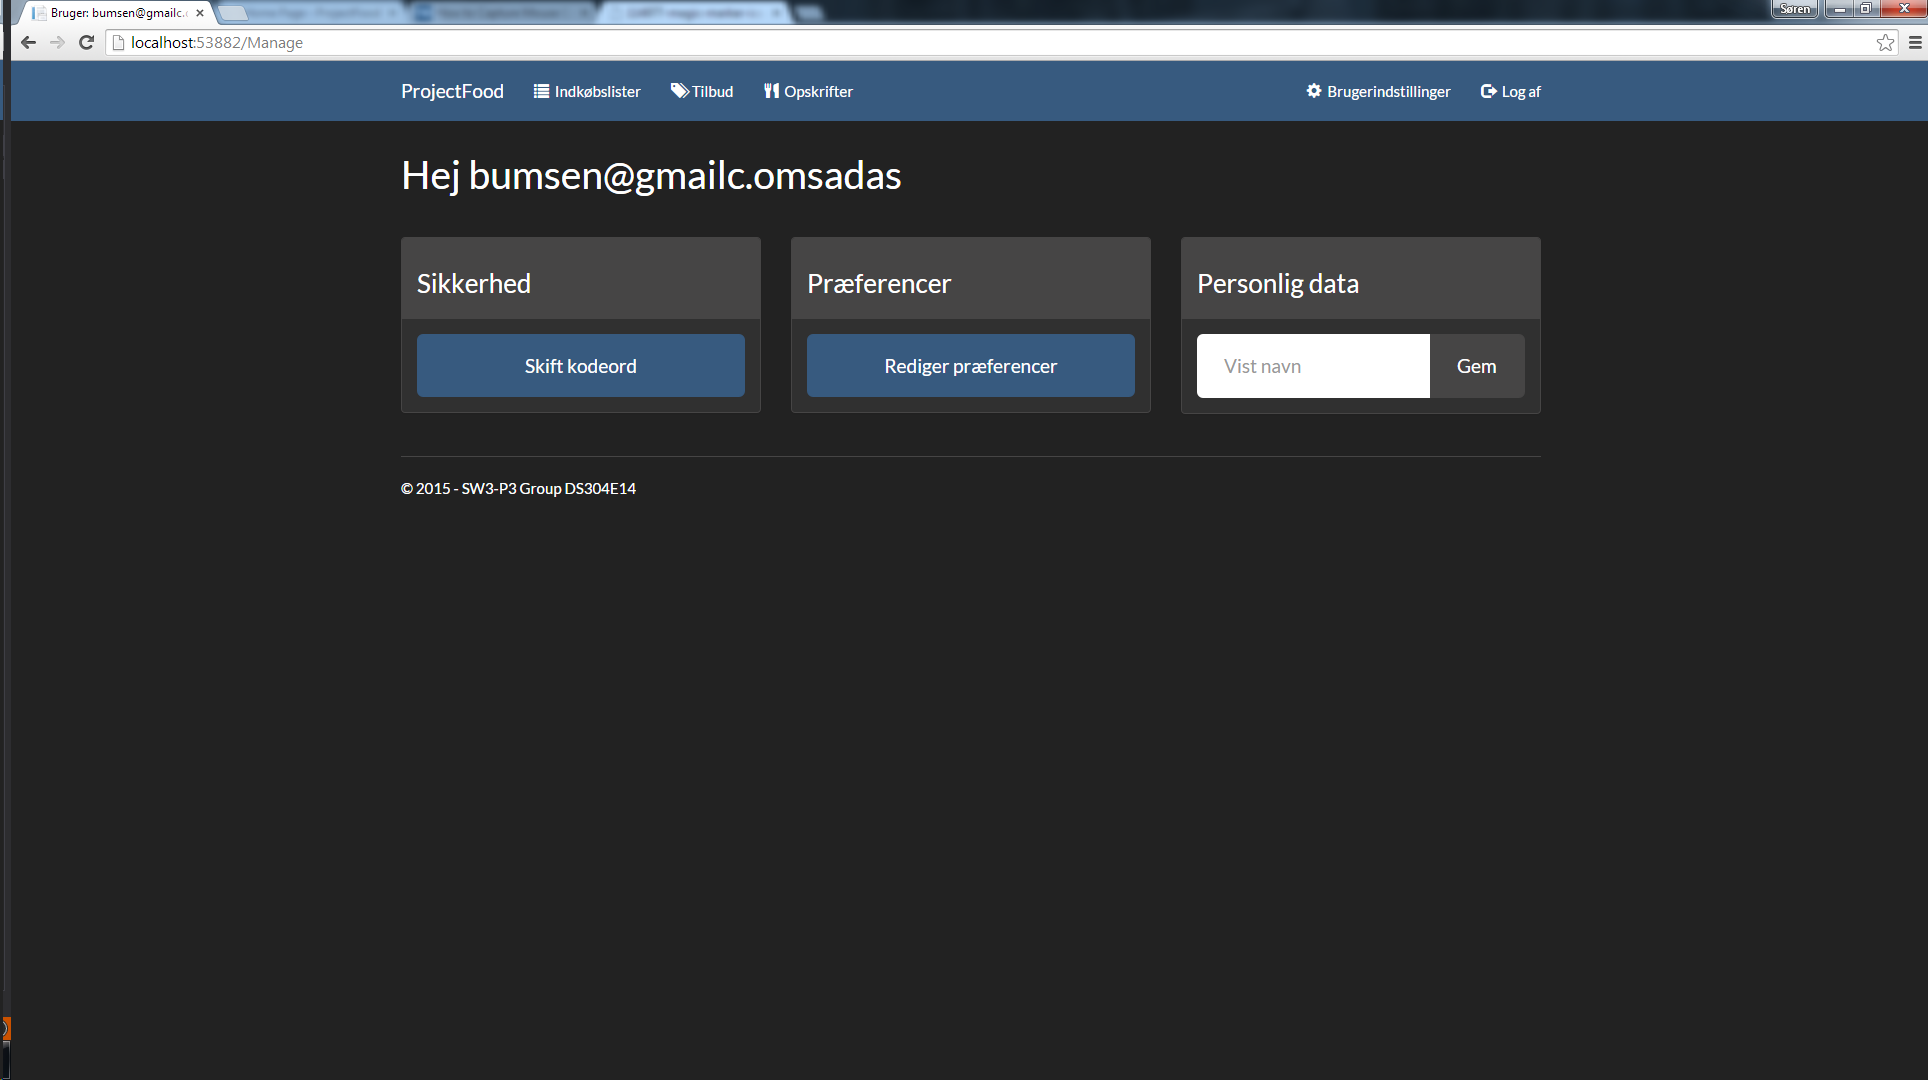
\includegraphics[width=0.9\textwidth,height=0.9\textheight,keepaspectratio, trim={1cm 0 0 16mm}, clip]{images/Screenshots/SettingsOld.png} \vspace{2 mm} $\rightarrow$ 
	 
	 Første test:
	 \begin{itemize}
	 	\item Reduceret antal klik
	 	\item Fjernet ordet Præferencer
	 	\item Forsøgt at give feedback
	 	\item Seriøs
	 \end{itemize}
	 Sidste test:
	 \begin{itemize}
	 	\item Nogle så ikke det blev gemt første gang
	 \end{itemize}
	 
	\end{column}
	\begin{column}{0.5\textwidth}
	 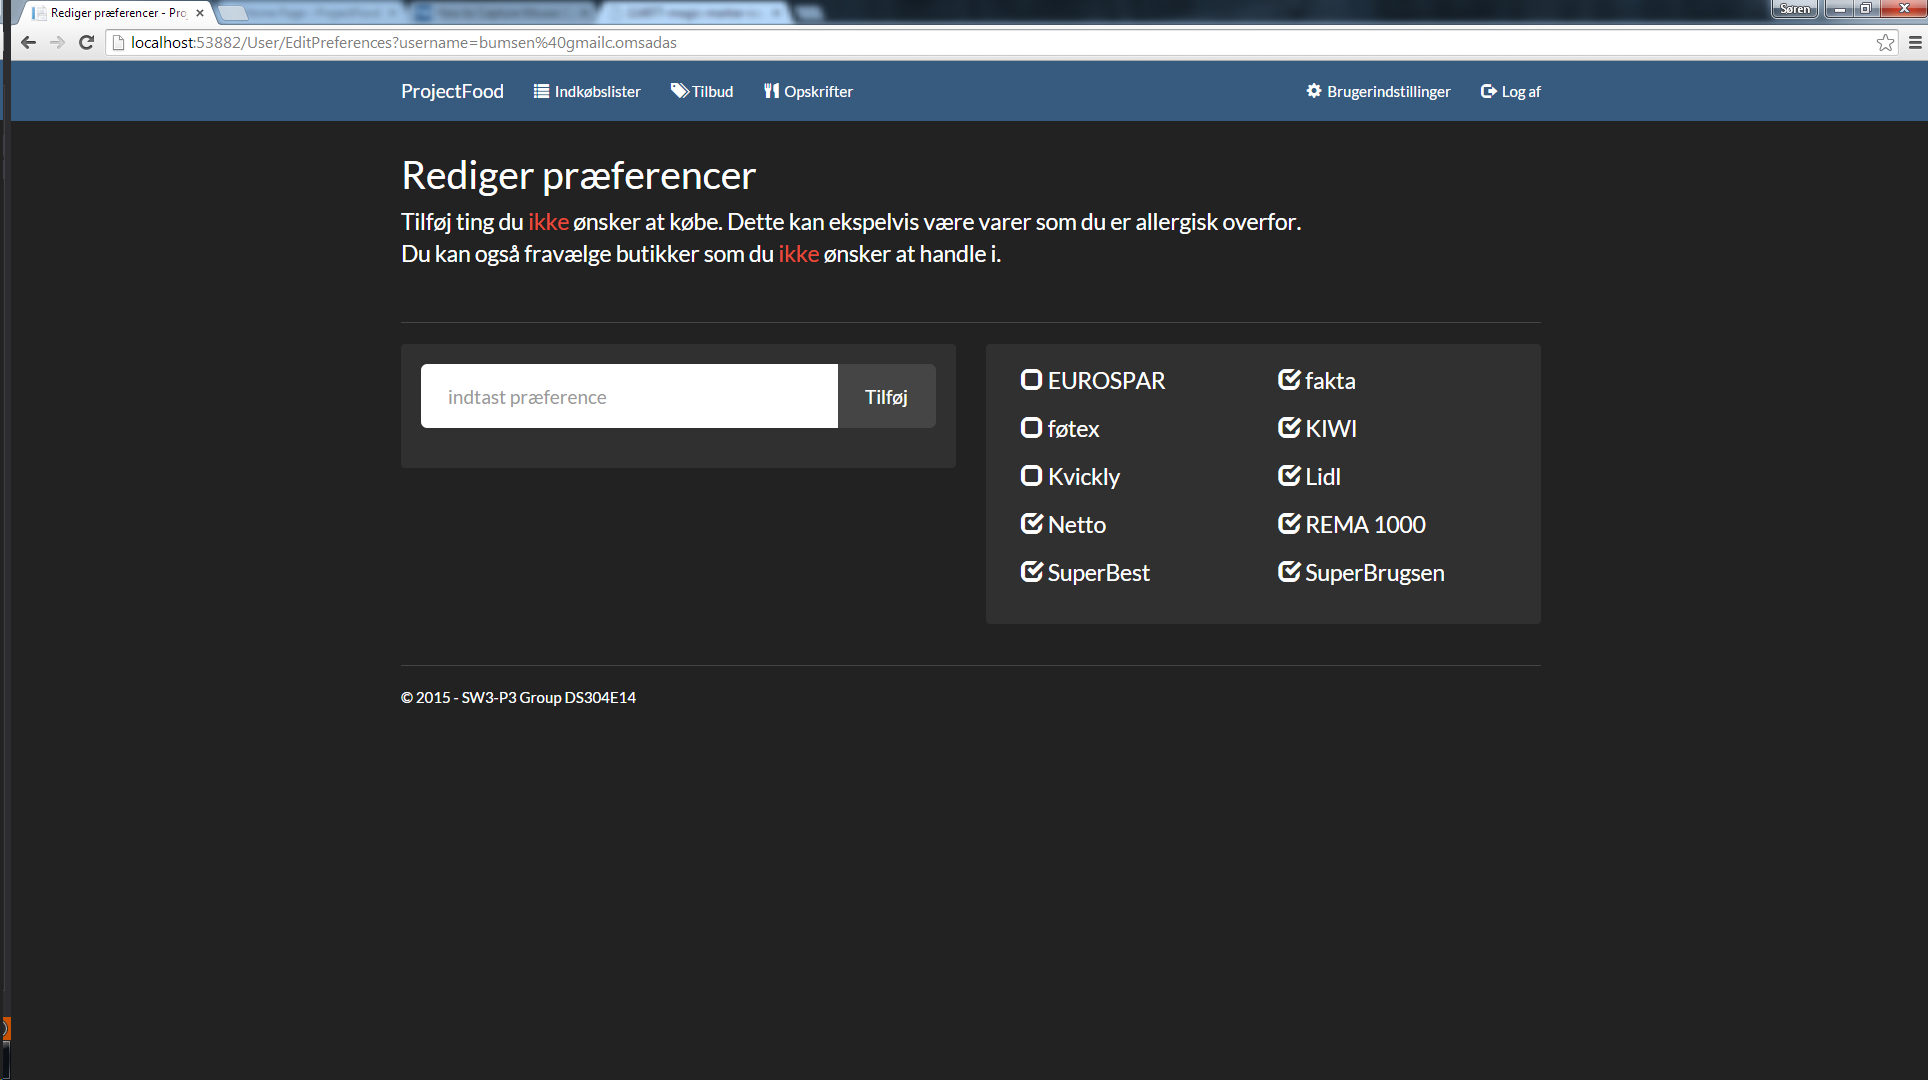
\includegraphics[width=1\textwidth,height=1\textheight,keepaspectratio, trim={1cm 0 0 16mm}, clip]{images/Screenshots/SettingsOld2.png}
	 
	 \vspace{2 mm}
	  
	  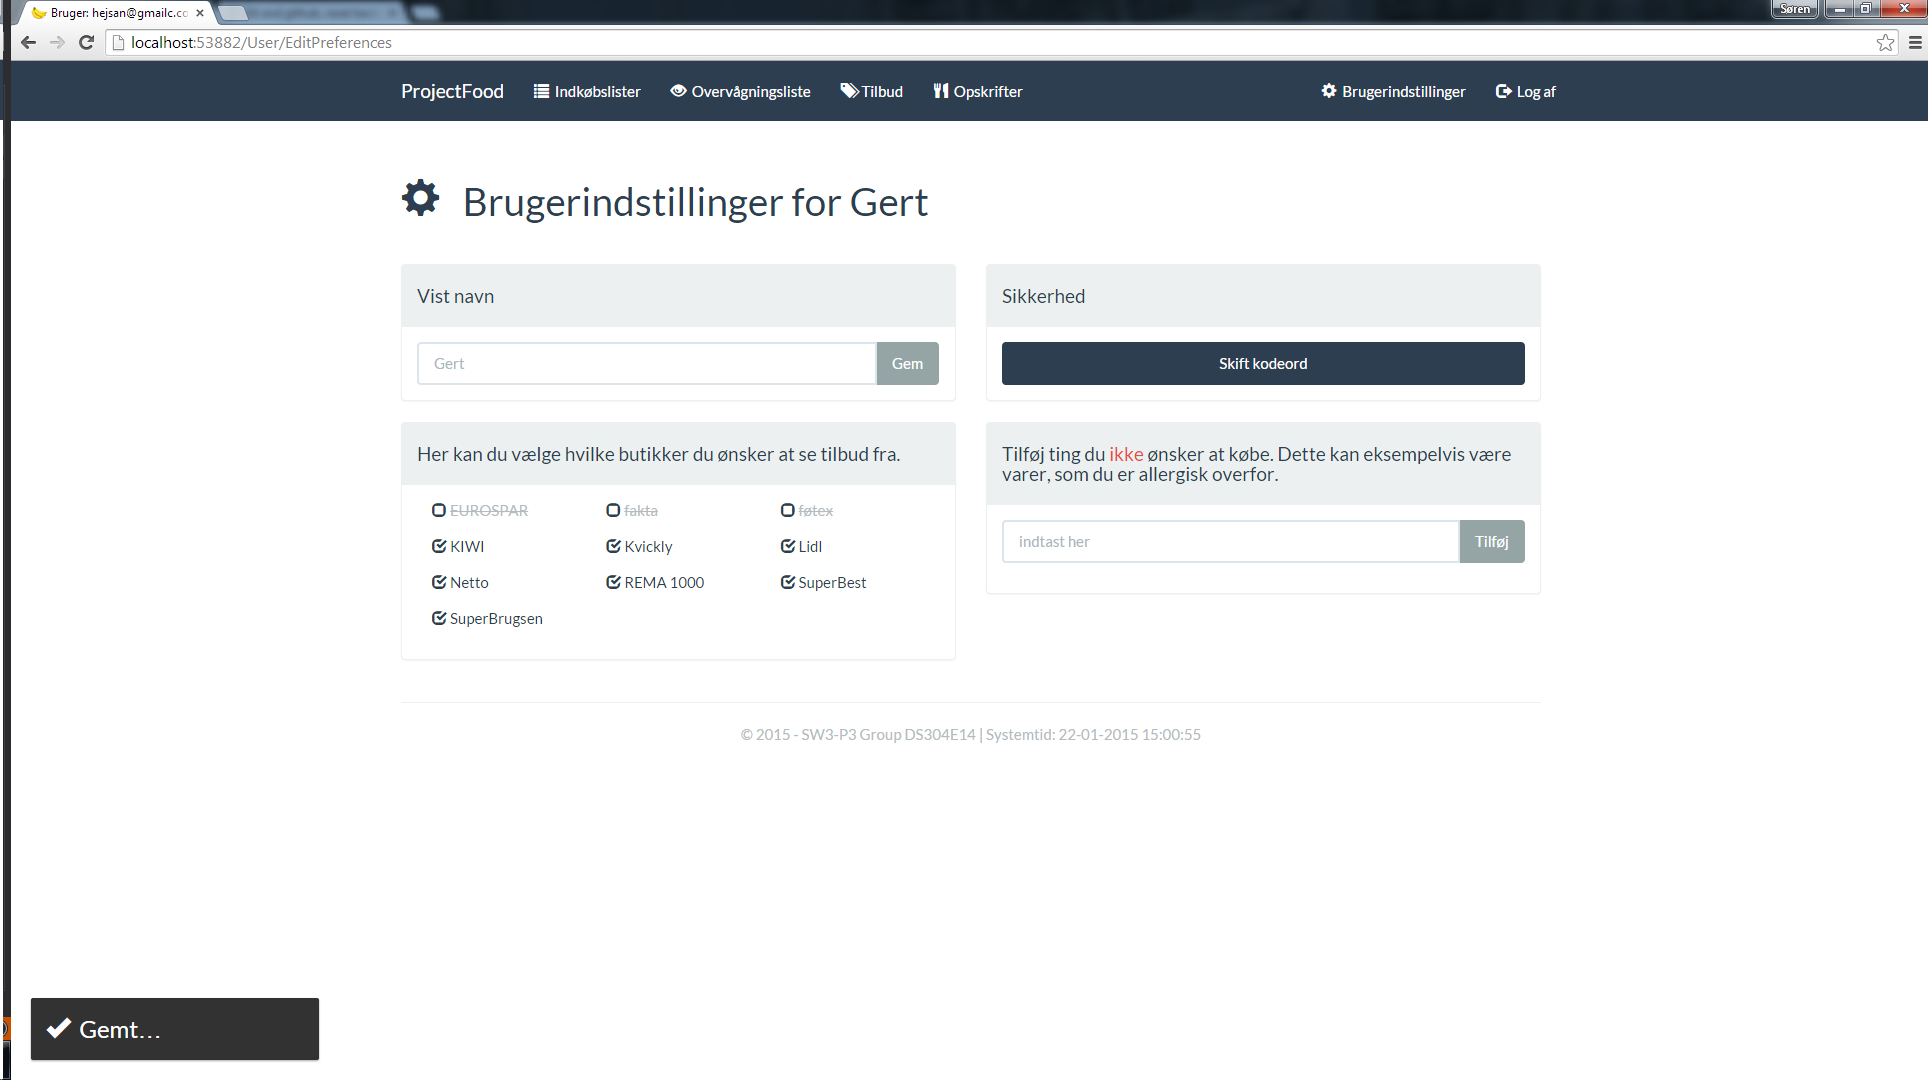
\includegraphics[width=1\textwidth,height=1\textheight,keepaspectratio, trim={1cm 0 0 16mm}, clip]{images/Screenshots/Settings.png}
	\end{column}
	\end{columns}
	

  \end{minipage}
	
\end{frame}

\begin{frame}{Resultater}
\framesubtitle{Indstillinger}


	
	\begin{minipage}[0.3\textheight]{\textwidth}
	\begin{columns}[T]
	\begin{column}{1\textwidth}
	
	\vspace{-15 pt}
	 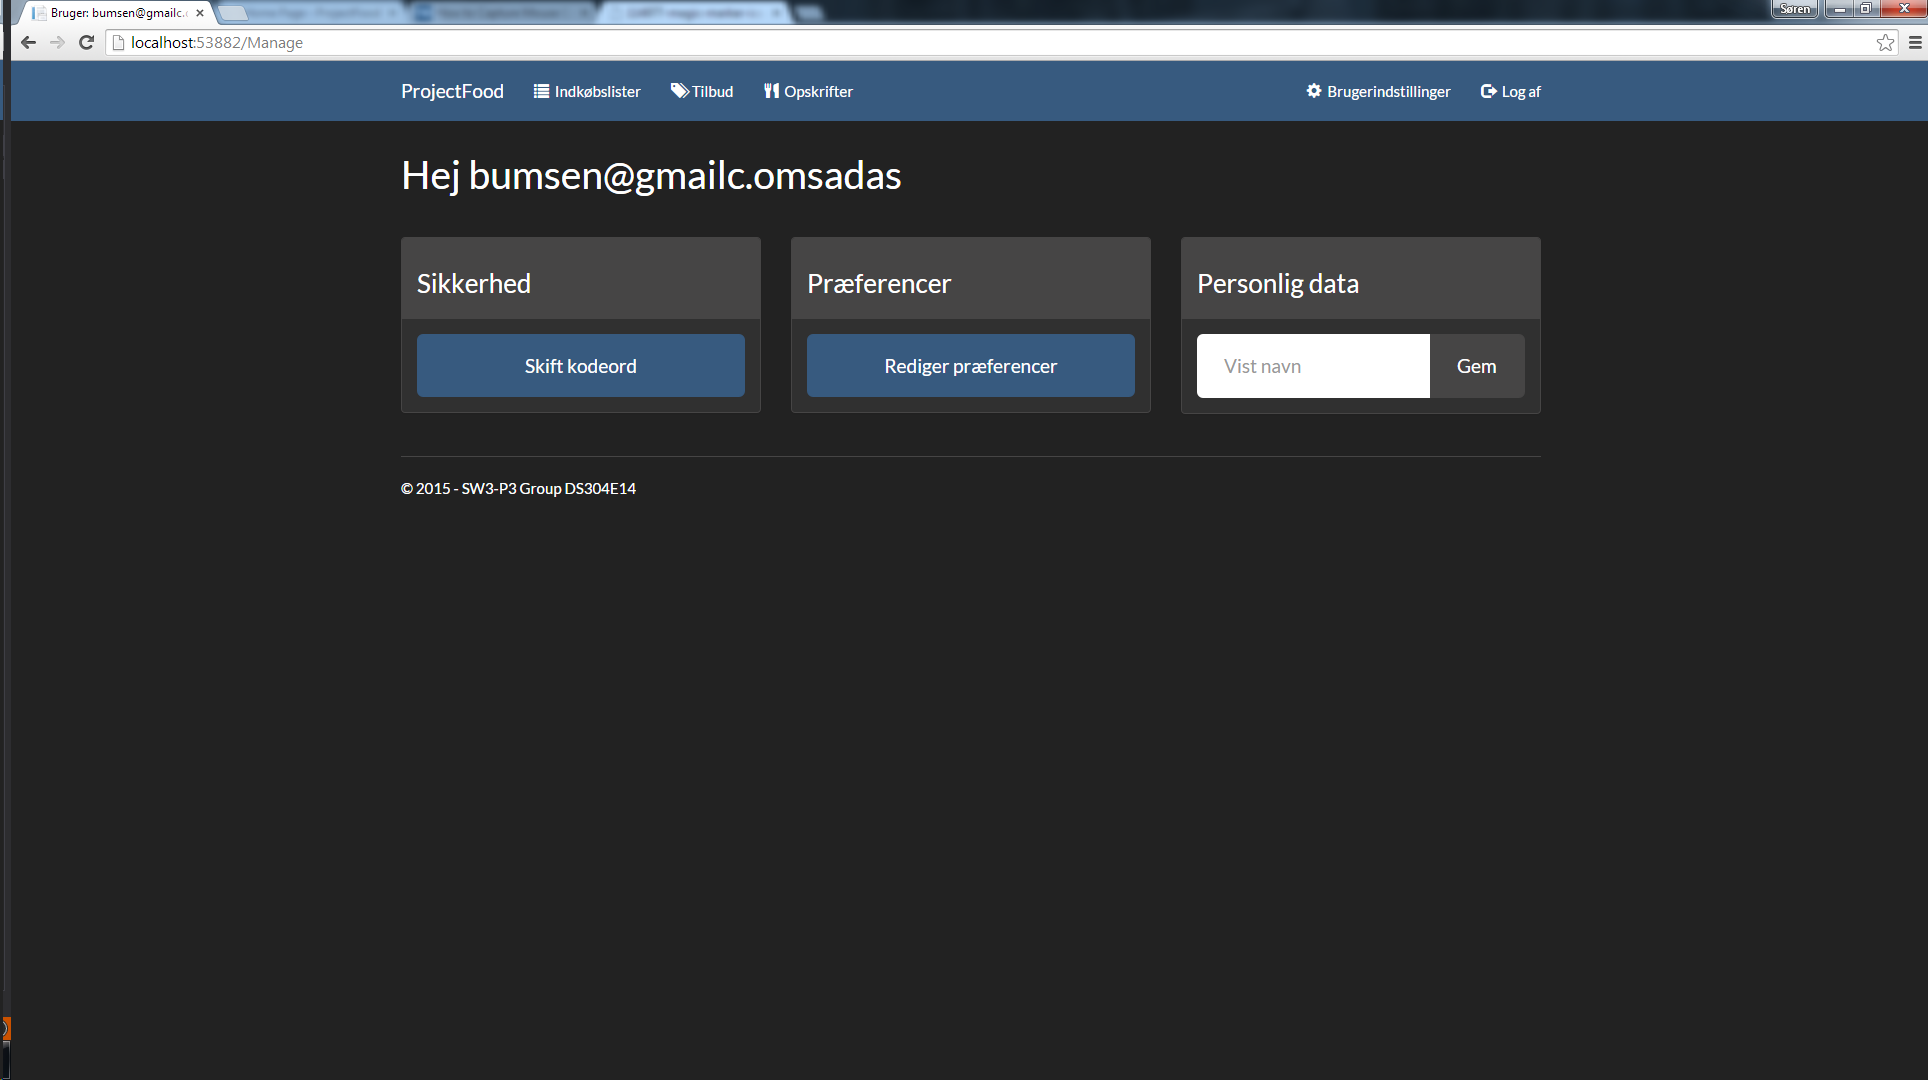
\includegraphics[width=1\textwidth,height=1\textheight,keepaspectratio, trim={1cm 0 0 16mm}, clip]{images/Screenshots/SettingsOld.png}
	 
	 \begin{itemize}
	 		 	\item Reduceret antal klik
	 		 	\item Fjernet ordet Præferencer
	 \end{itemize}
	
	\end{column}

	\end{columns}

  \end{minipage}
	
\end{frame}
\begin{frame}{Resultater}
\framesubtitle{Indstillinger}


	
	\begin{minipage}[0.3\textheight]{\textwidth}
	\begin{columns}[T]
	\begin{column}{1\textwidth}
	\vspace{-15 pt}
	 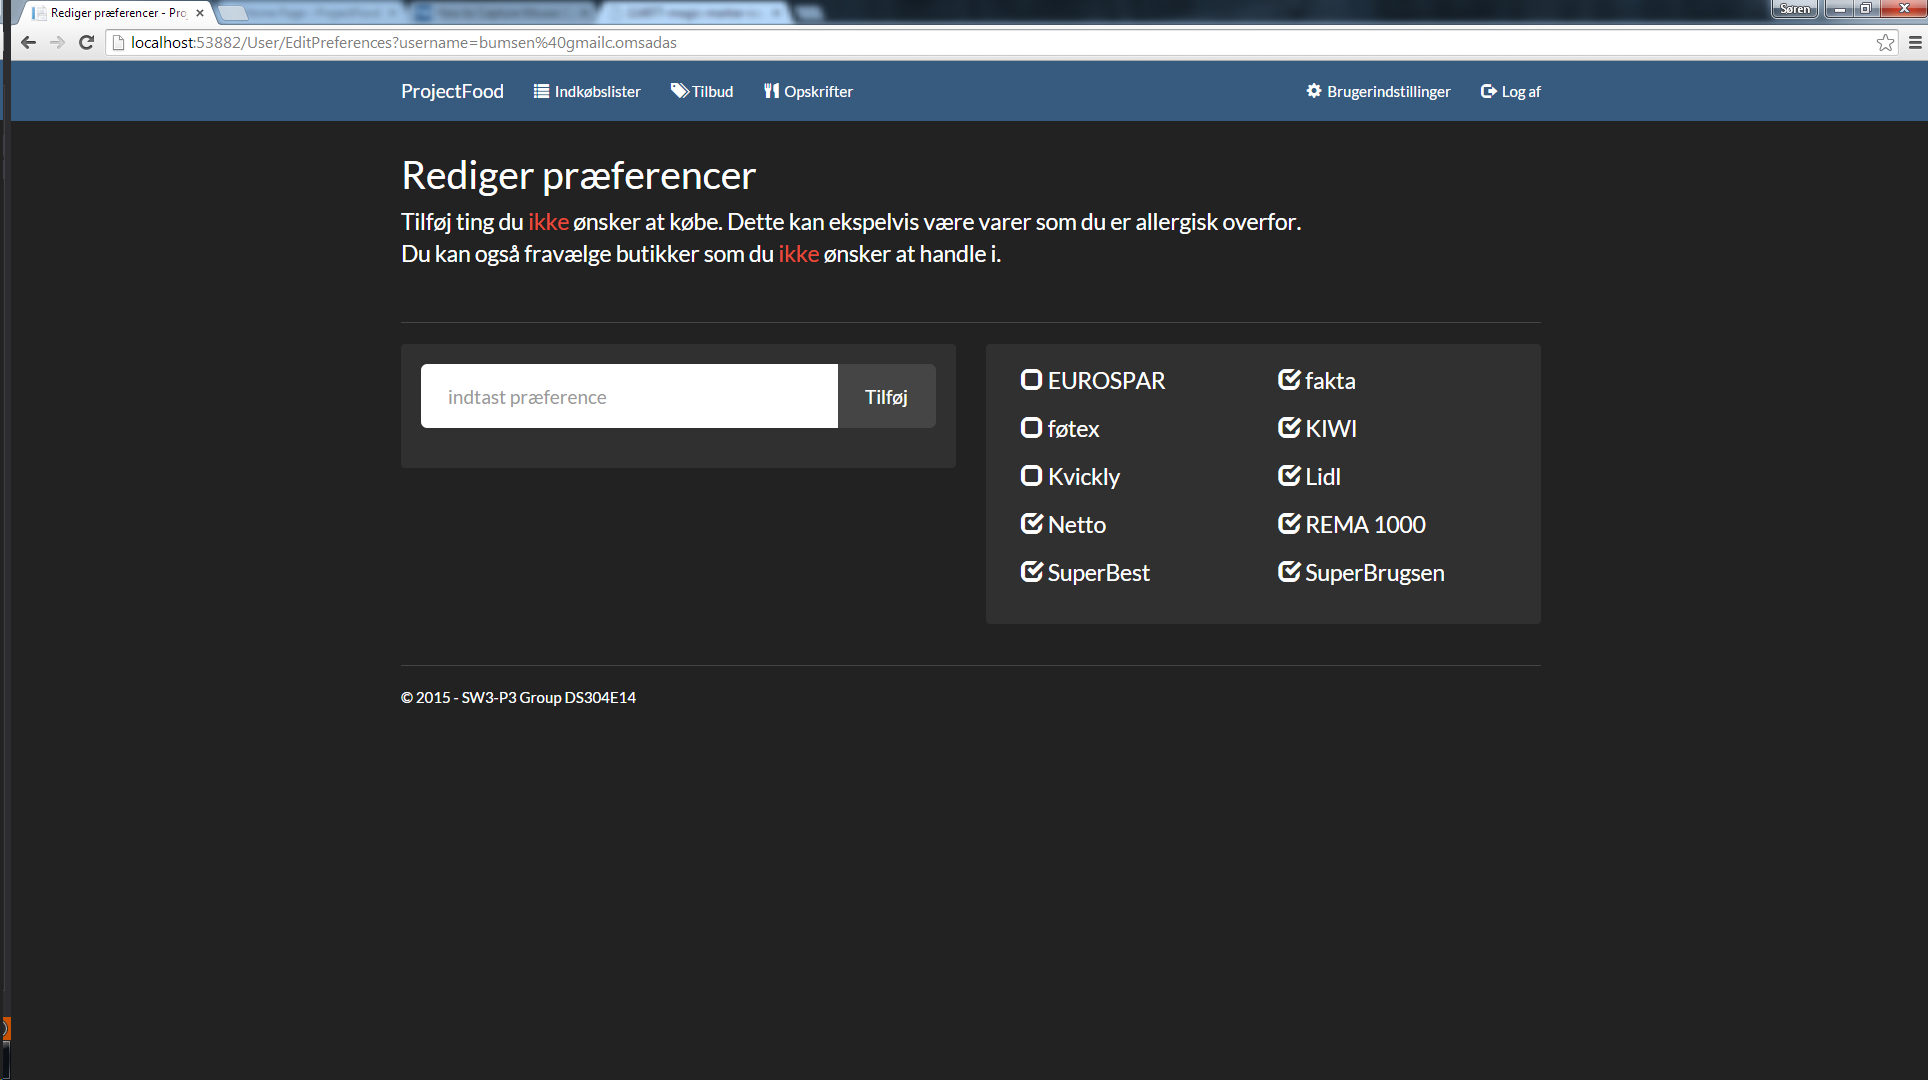
\includegraphics[width=1\textwidth,height=1\textheight,keepaspectratio, trim={1cm 0 0 16mm}, clip]{images/Screenshots/SettingsOld2.png}
	 
	 \begin{itemize}
	 	 	\item Var i tvivl om man havde gemt
	 	 	\item Seriøs
	 \end{itemize}
	
	\end{column}

	\end{columns}

  \end{minipage}
	
\end{frame}

\begin{frame}{Resultater}
\framesubtitle{Indstillinger}


	
	\begin{minipage}[0.3\textheight]{\textwidth}
	\begin{columns}[T]
	\begin{column}{1\textwidth}
	\vspace{-15 pt}
	 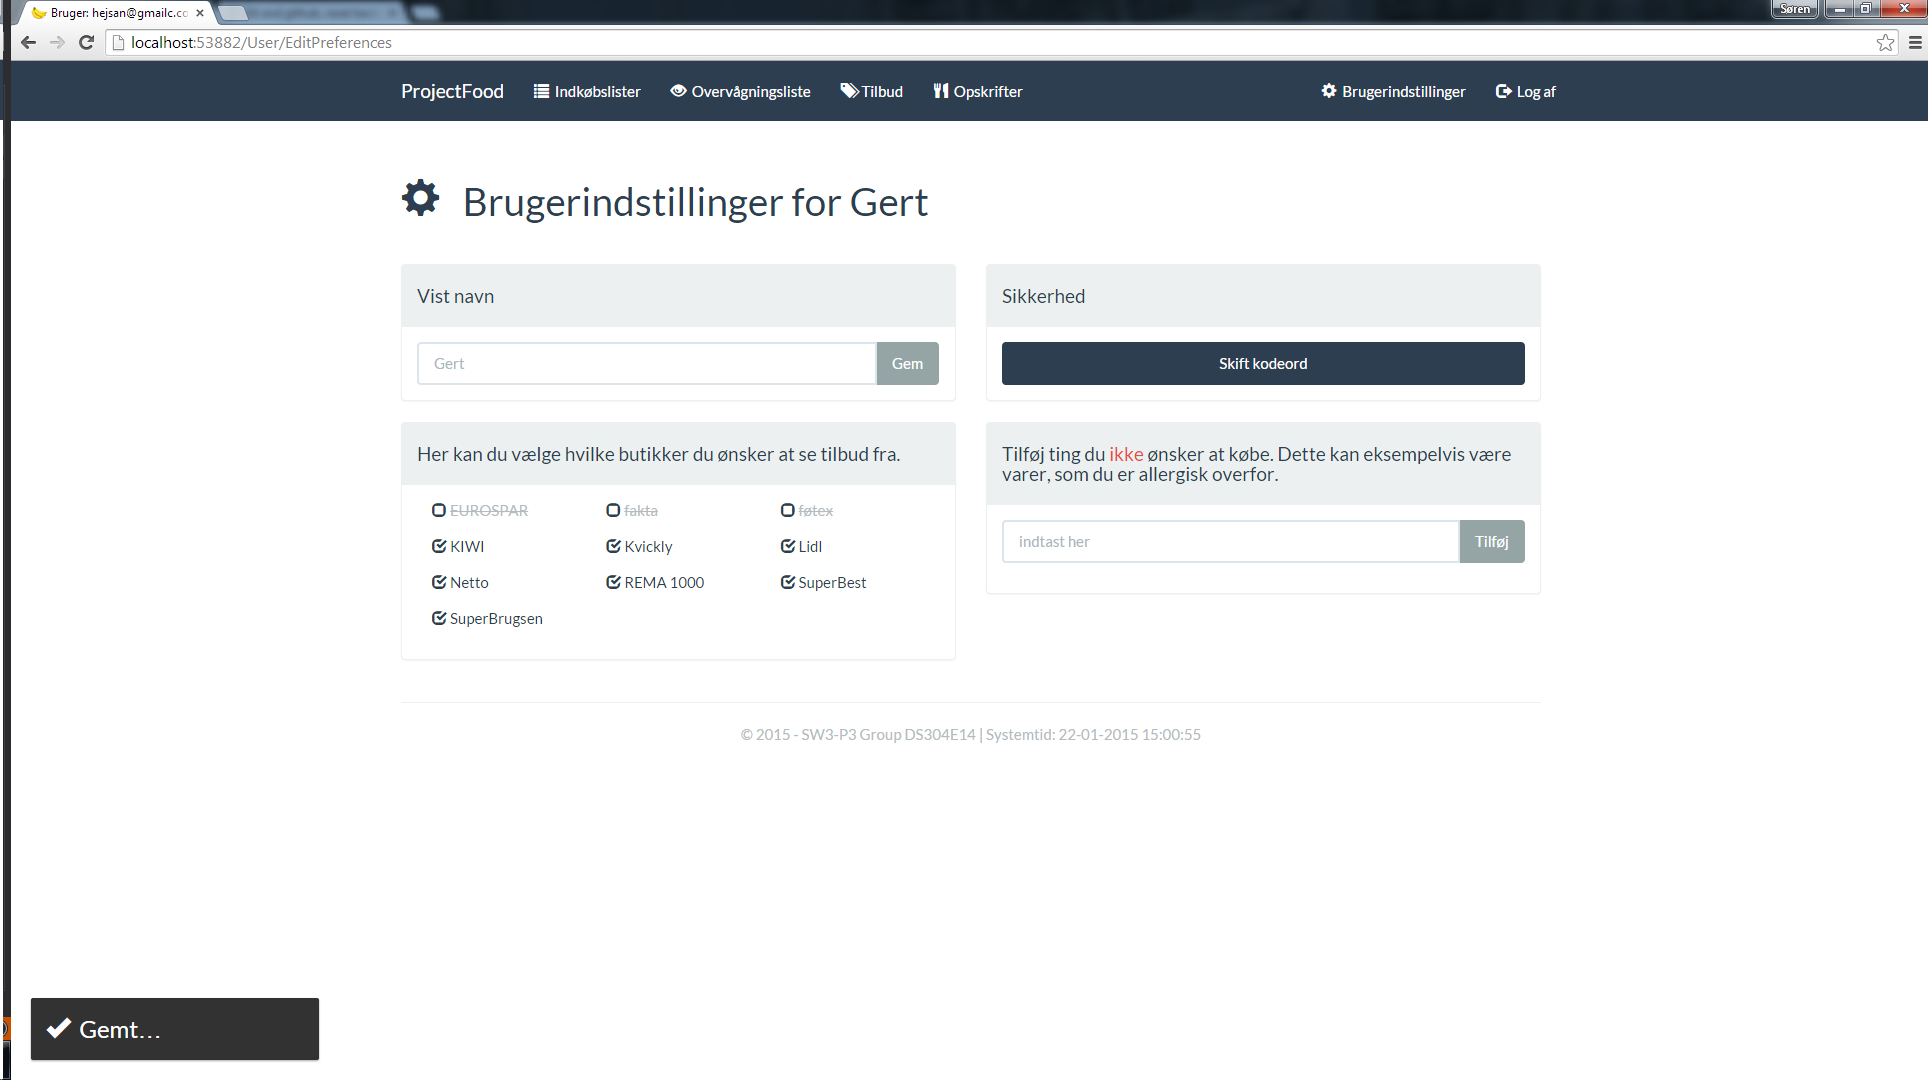
\includegraphics[width=1\textwidth,height=1\textheight,keepaspectratio, trim={1cm 0 0 16mm}, clip]{images/Screenshots/Settings.png}
	
	\begin{itemize}
		\item Snackbar
		\item Hjalp lidt
	\end{itemize}
	\end{column}

	\end{columns}

  \end{minipage}
	
\end{frame}
\begin{frame}{Resultater}
\framesubtitle{Indkøbsliste}
	\subsubsection{Indkøbsliste}
	
	\begin{minipage}[0.3\textheight]{\textwidth}
	\begin{columns}[T]
	\begin{column}{0.5\textwidth}
	 
	 Første test
	 \begin{itemize}
	 	\item Viser altid ikon nu
	 	\item Adskillelse af input bokse
	 	\item Konsistente farver for vælg tilbud
	 	\item Udstregning blev ikke brugt
	 \end{itemize}
	 Sidste test
	 \begin{itemize}
	 	\item Udstregning stadig ikke brugt
	 	\item Seriøs
	 \end{itemize}
	 
	\end{column}
	\begin{column}{0.5\textwidth}
	 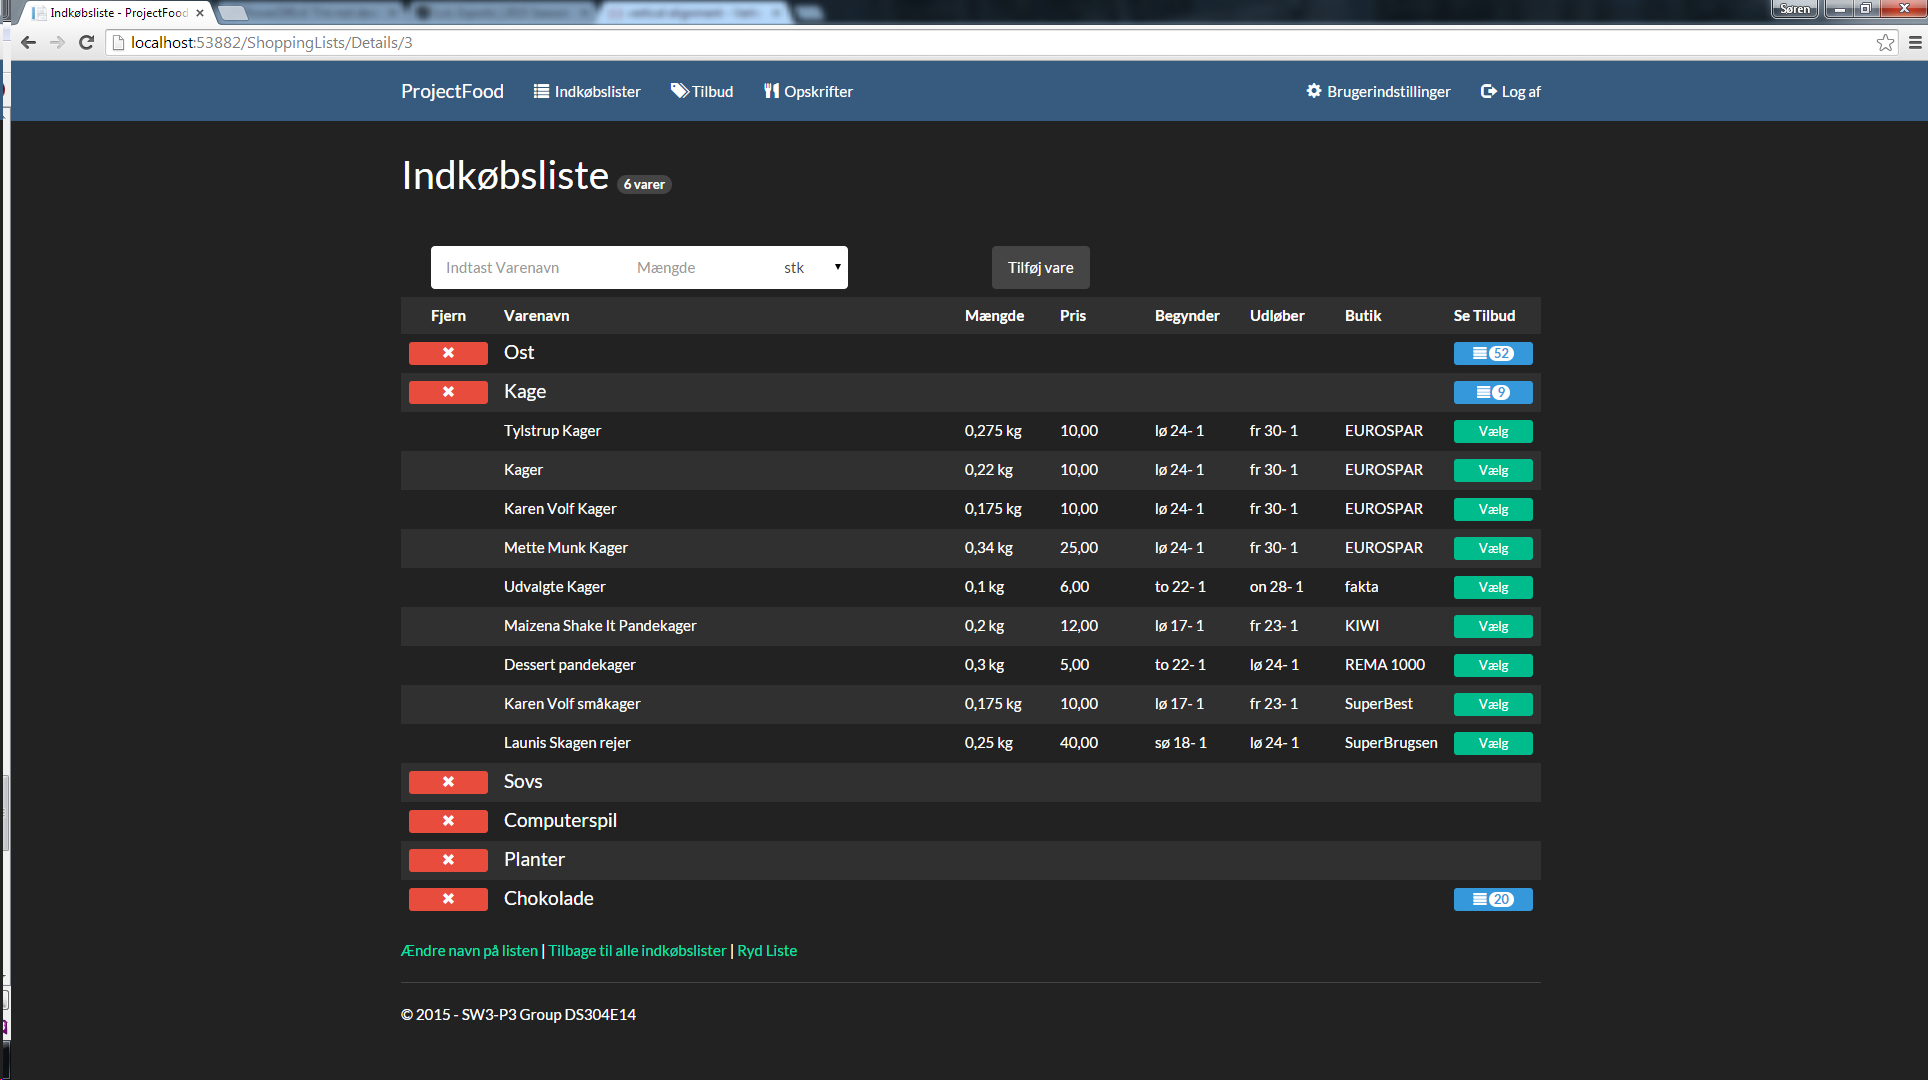
\includegraphics[width=1\textwidth,height=1\textheight,keepaspectratio, trim={1cm 0 0 16mm}, clip]{images/Screenshots/ShoppingListOffersOld.png}
	 
	 \vspace{2 mm}
	  
	  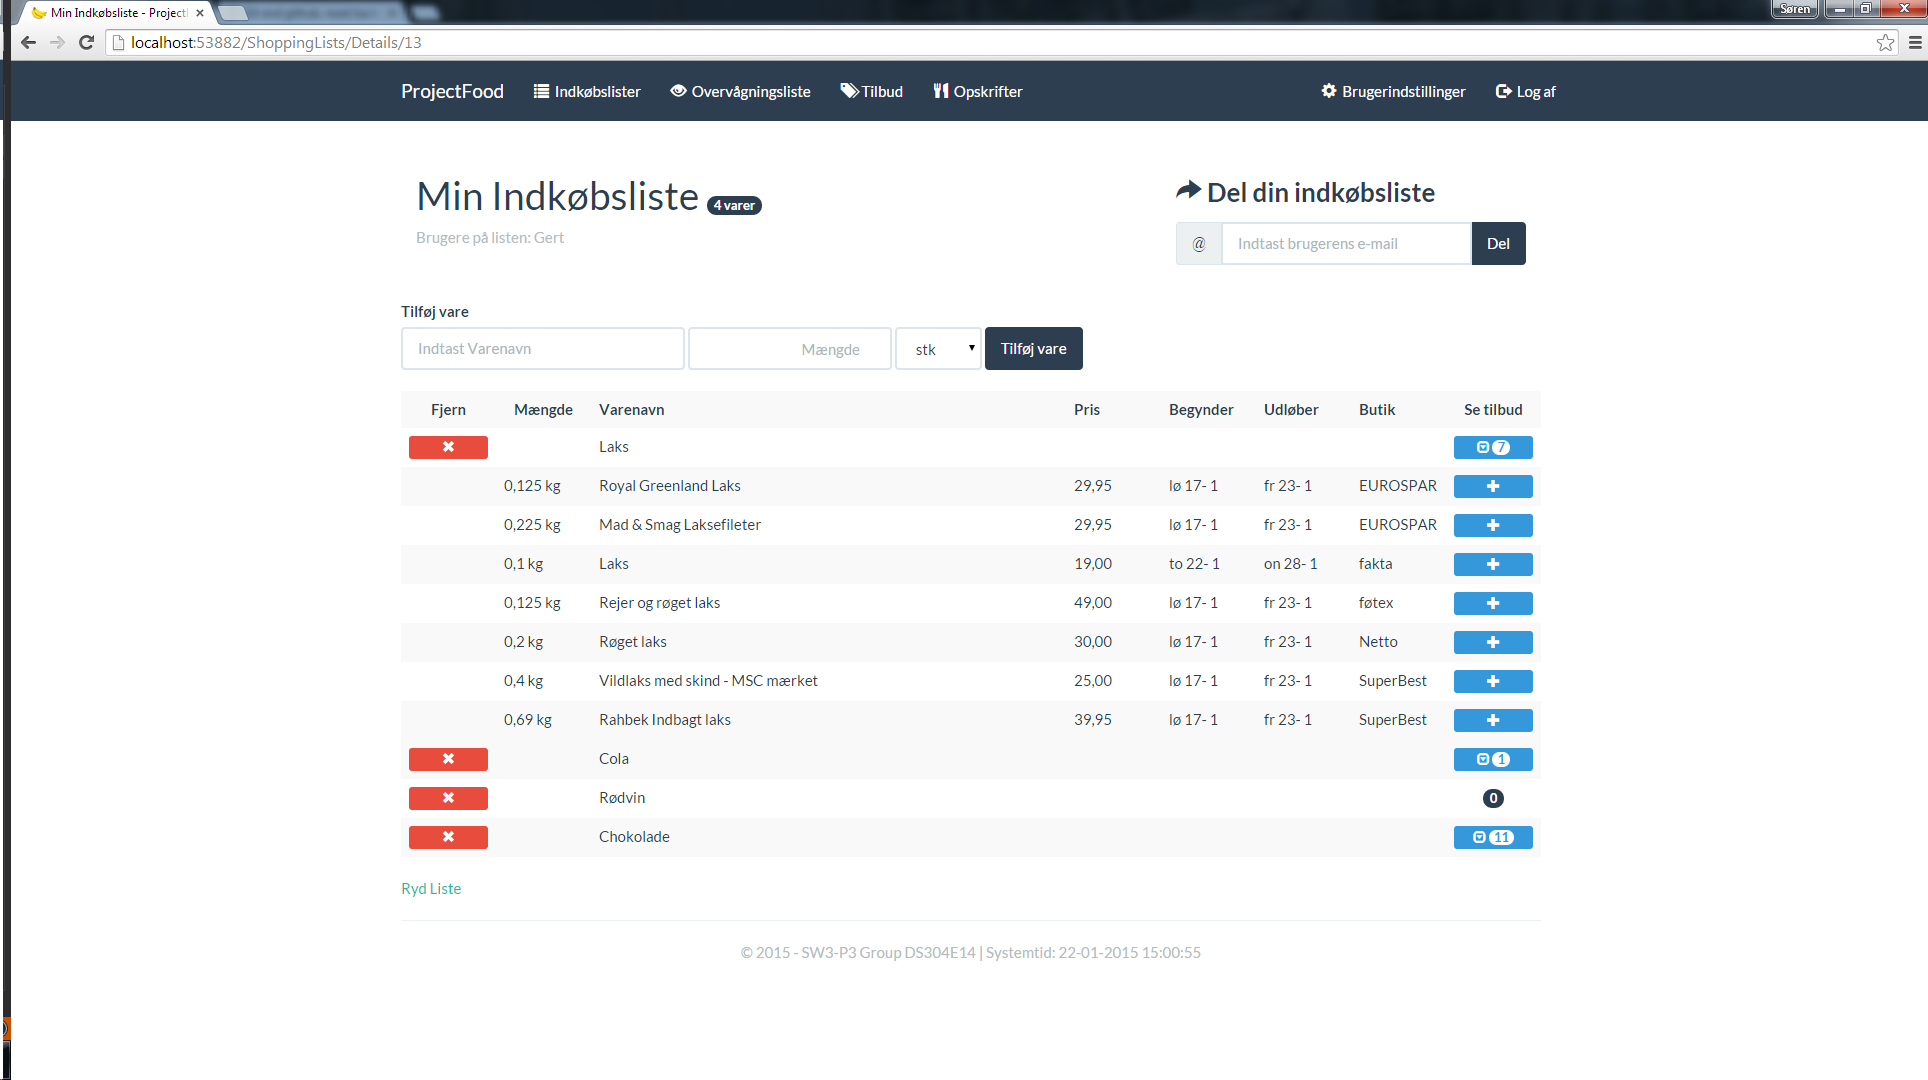
\includegraphics[width=1\textwidth,height=1\textheight,keepaspectratio, trim={1cm 0 0 16mm}, clip]{images/Screenshots/ShoppingList.png}
	\end{column}
	\end{columns}
	

  \end{minipage}
	
\end{frame}
\begin{frame}{Resultater}
\framesubtitle{Indkøbsliste}

	\begin{minipage}[0.3\textheight]{\textwidth}
	\begin{columns}[T]
	\begin{column}{1\textwidth}
	 \vspace{-15 pt}
	 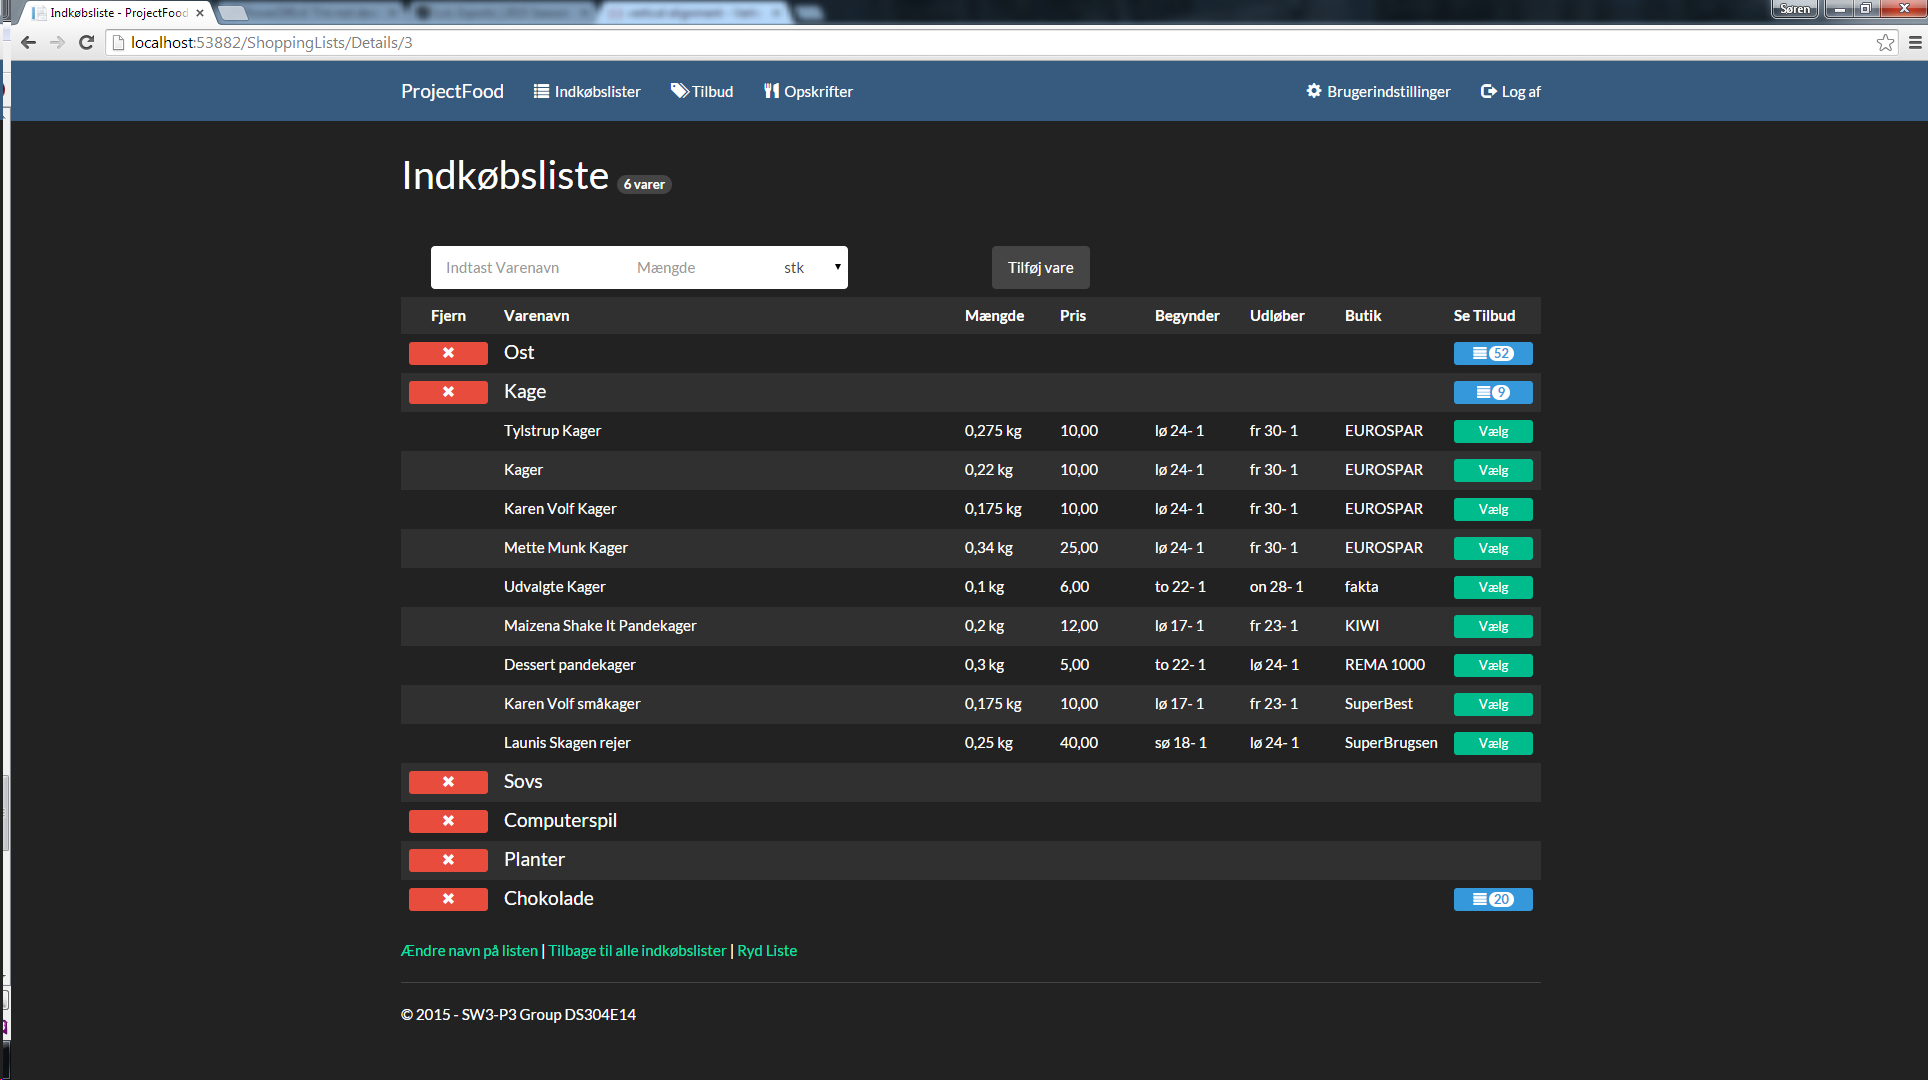
\includegraphics[width=1\textwidth,height=1\textheight,keepaspectratio, trim={1cm 0 0 16mm}, clip]{images/Screenshots/ShoppingListOffersOld.png}
	
	\begin{itemize}
		\item Ikke konsistent
		\item En boks med input
	\end{itemize}
	\end{column}

	\end{columns}

  \end{minipage}
	
\end{frame}
\begin{frame}{Resultater}
\framesubtitle{Indkøbsliste}

	\begin{minipage}[0.3\textheight]{\textwidth}
	\begin{columns}[T]
	\begin{column}{1\textwidth}
	\vspace{-15 pt}
	 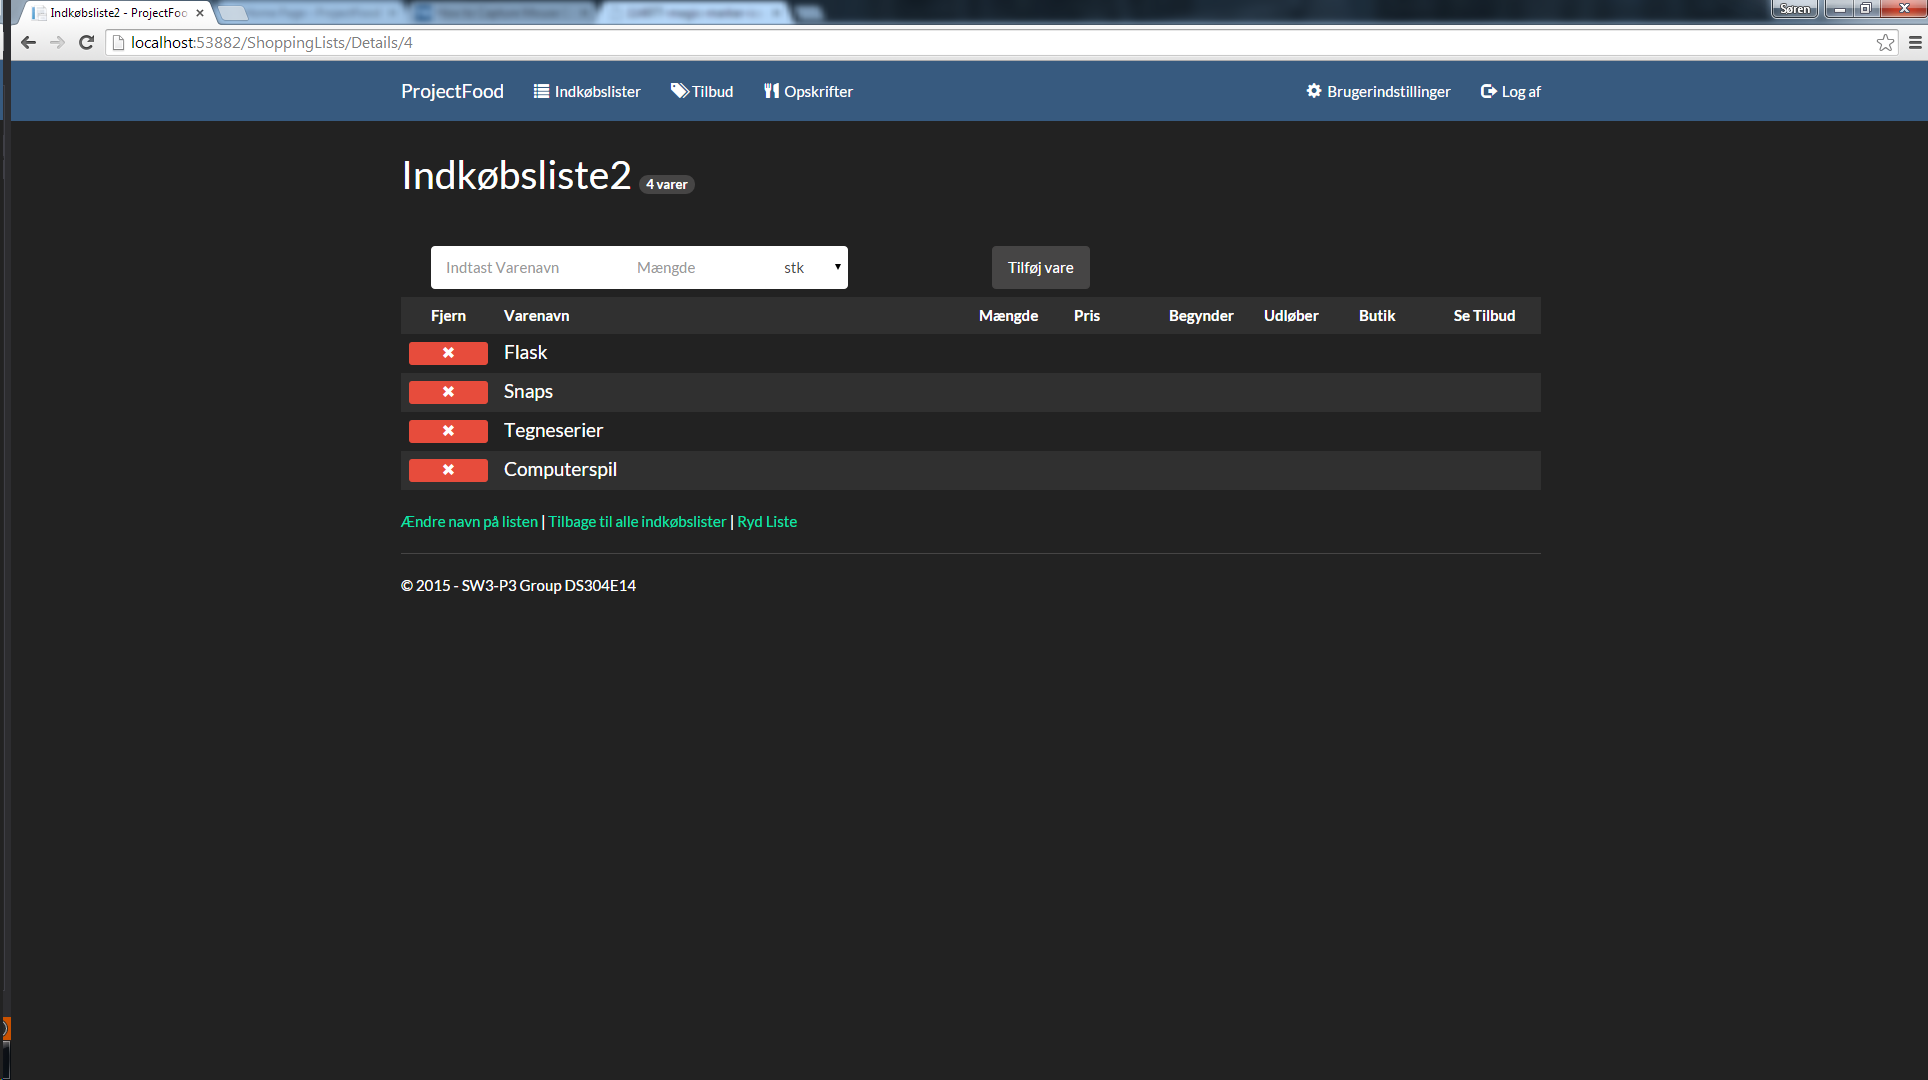
\includegraphics[width=1\textwidth,height=1\textheight,keepaspectratio, trim={1cm 0 0 16mm}, clip]{images/Screenshots/ShoppingListOld.png}
	 
	 \begin{itemize}
	 	\item Problem når der ingen tilbud var
	 \end{itemize}
	
	\end{column}

	\end{columns}

  \end{minipage}
	
\end{frame}
\begin{frame}{Resultater}
\framesubtitle{Indkøbsliste}


	
	\begin{minipage}[0.3\textheight]{\textwidth}
	\begin{columns}[T]
	\begin{column}{1\textwidth}
	
	 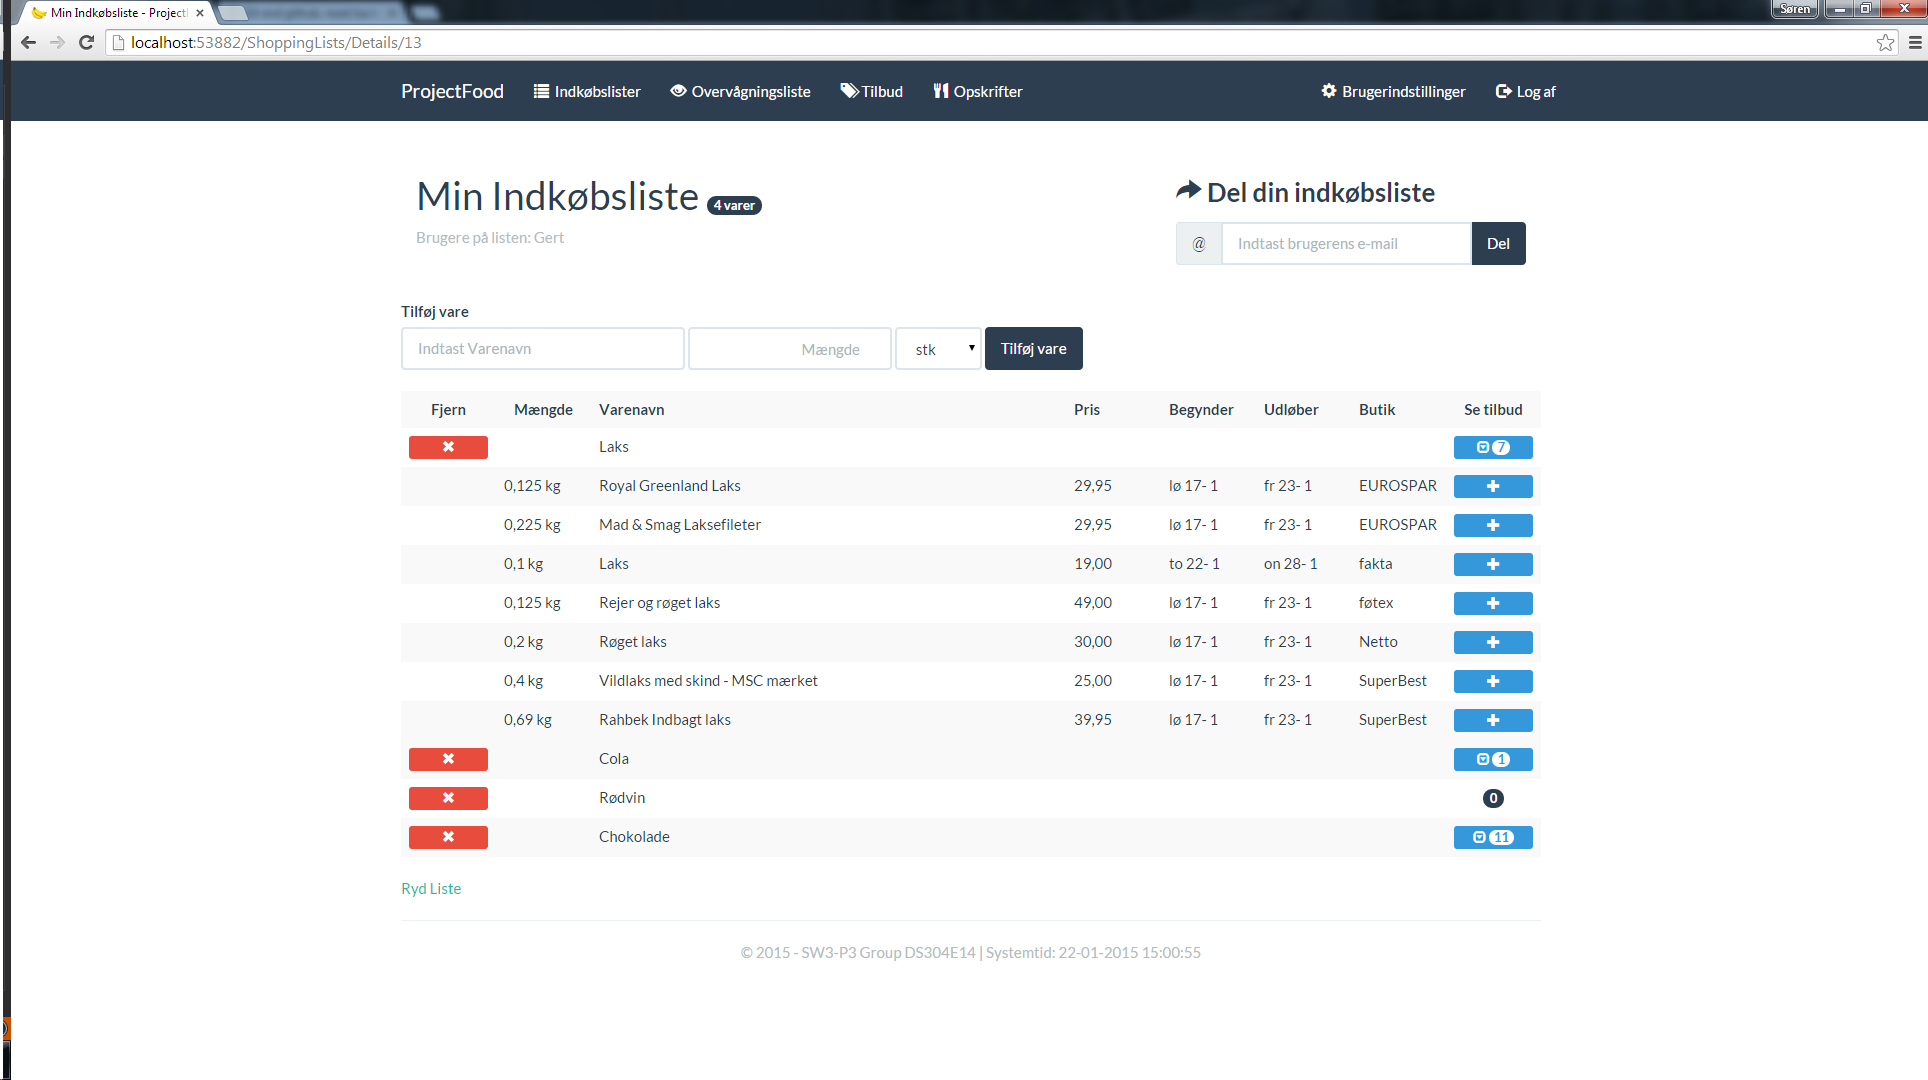
\includegraphics[width=1\textwidth,height=1\textheight,keepaspectratio, trim={1cm 0 0 16mm}, clip]{images/Screenshots/ShoppingList.png}
	 
	 \begin{itemize}
	 	\item Udstregning stadig ikke brugt
	 	\item Konsistente ikoner
	 	\item Proximity på boksen
	 	\item Viser altid ikon 
	 \end{itemize}
	
	\end{column}

	\end{columns}

  \end{minipage}
	
\end{frame}

\begin{frame}{Resultater}
\framesubtitle{Oversigt over Opskrifter}
	\subsubsection{Oversigt over Opskrifter}
	
	\begin{minipage}[0.3\textheight]{\textwidth}
	\begin{columns}[T]
	\begin{column}{0.5\textwidth}
	
	Første test:
	\begin{itemize}
	\item Mouseover
	\item Ingen kunne navigere ind på opskriften uden først at blive i tvivl om hvordan.
	\item Kritisk
	
	\end{itemize}
	Sidste test:
	\begin{itemize}
		\item Ingen problemer her
	\end{itemize}
	
	\end{column}
	\begin{column}{0.5\textwidth}
	 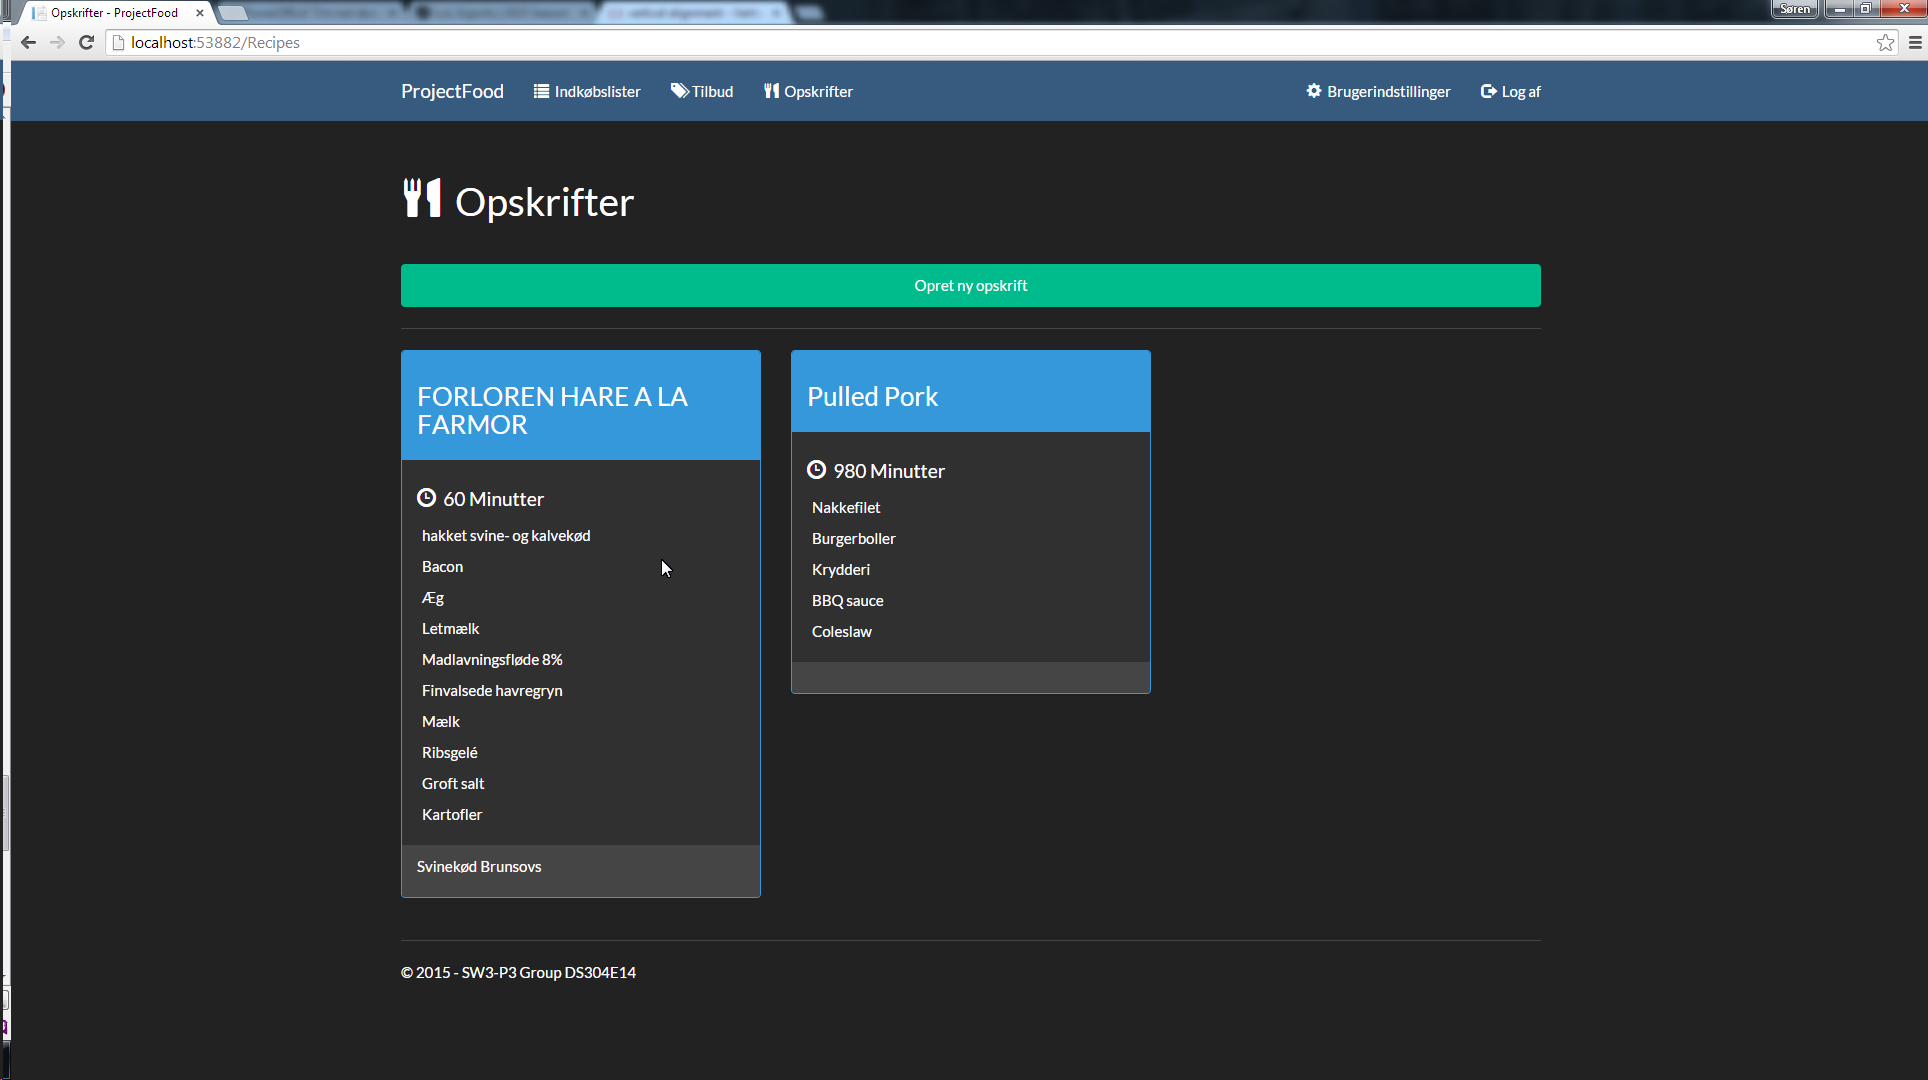
\includegraphics[width=1\textwidth,height=1\textheight,keepaspectratio, trim={1cm 0 0 16mm}, clip]{images/Screenshots/RecipeOld.png}
	 
	 \vspace{2 mm}
	  
	  \includegraphics[width=1\textwidth,height=1\textheight,keepaspectratio, trim={1cm 0 0 16mm}, clip]{images/Screenshots//Recipe.png}
	\end{column}
	\end{columns}
	

  \end{minipage}
  
  	
\end{frame}

\begin{frame}{Resultater}
\framesubtitle{Oversigt over Opskrifter}

	
	\begin{minipage}[0.3\textheight]{\textwidth}
	\begin{columns}[T]
	\begin{column}{1\textwidth}
	 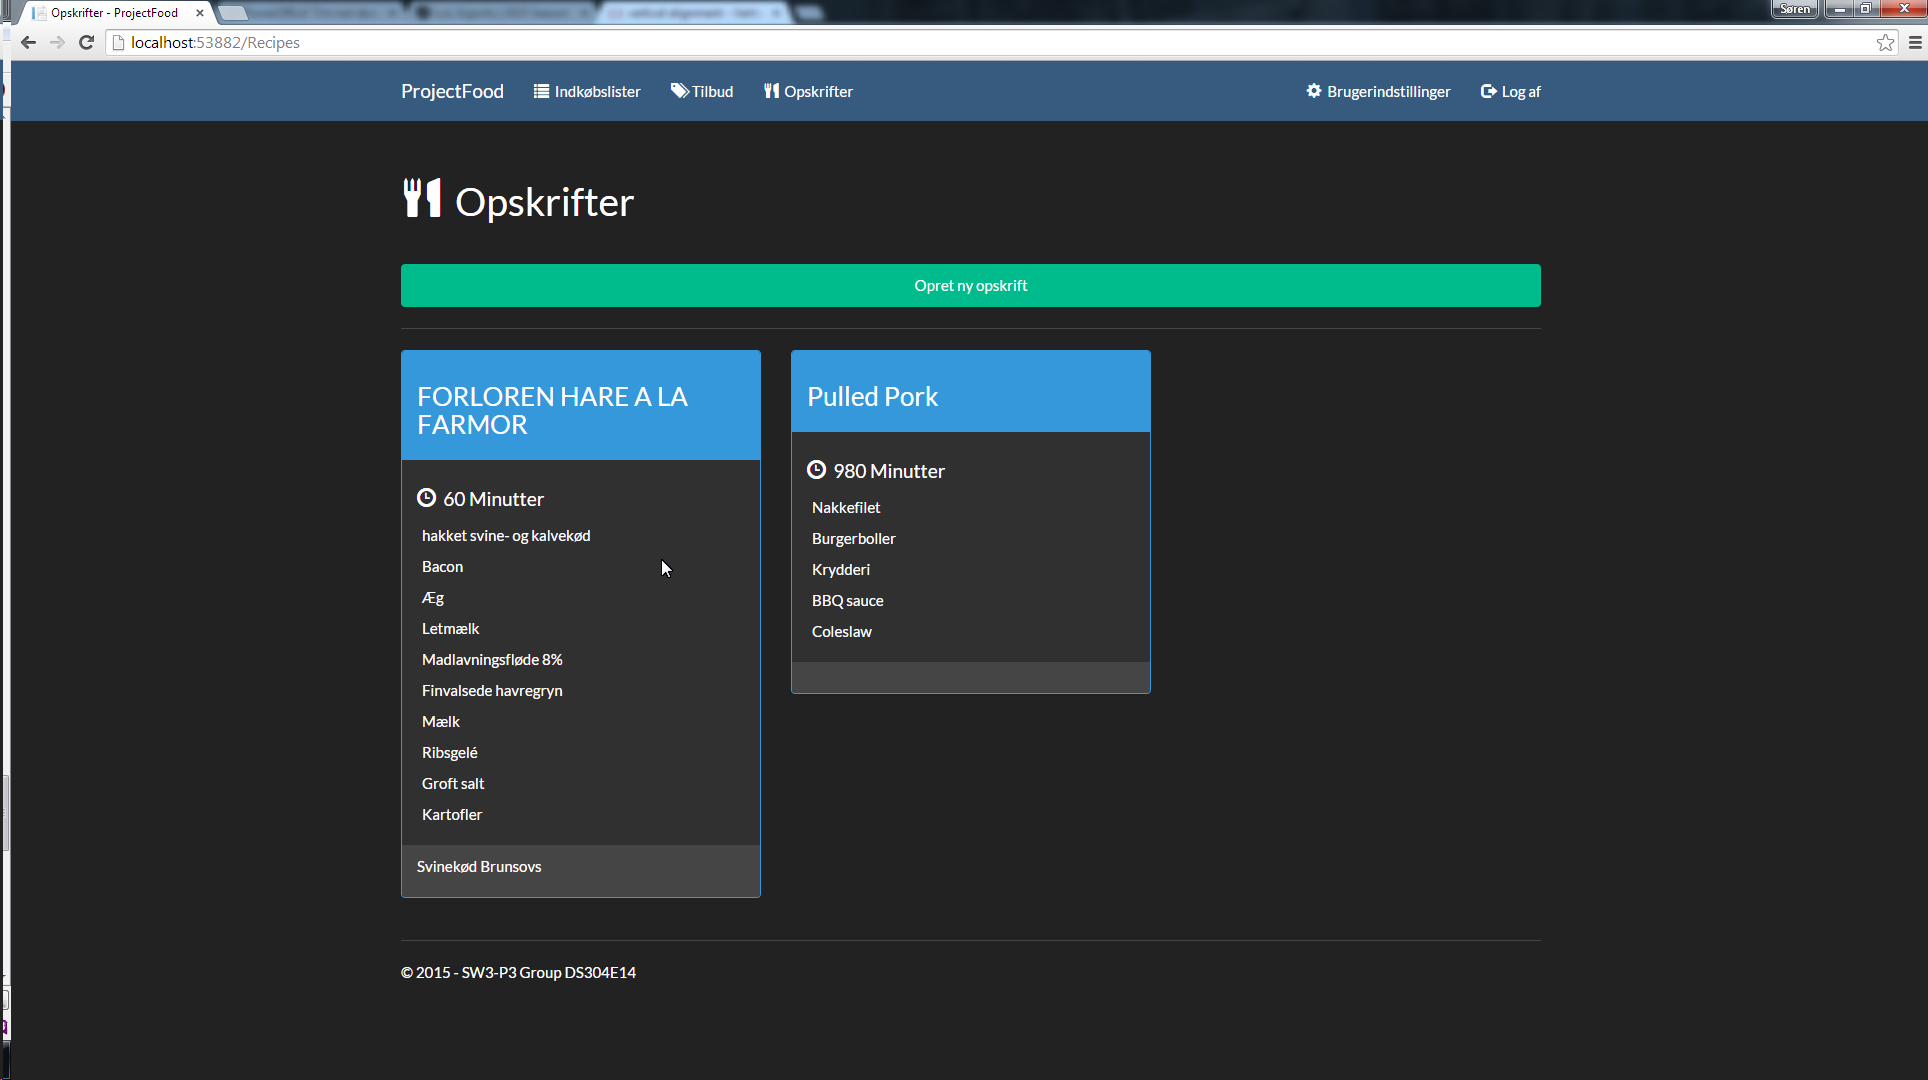
\includegraphics[width=1\textwidth,height=1\textheight,keepaspectratio, trim={1cm 0 0 16mm}, clip]{images/Screenshots/RecipeOld.png}
	 
	 	\begin{itemize}
	 	\item Mouseover
	 	\item Ingen kunne navigere ind på opskriften uden først at blive i tvivl om hvordan.
	 	\item Kritisk
	 	
	 	\end{itemize}
	
	\end{column}

	\end{columns}

  \end{minipage}
	
\end{frame}

\begin{frame}{Resultater}
\framesubtitle{Oversigt over Opskrifter}

	
	\begin{minipage}[0.3\textheight]{\textwidth}
	\begin{columns}[T]
	\begin{column}{1\textwidth}
	 \includegraphics[width=1\textwidth,height=1\textheight,keepaspectratio, trim={1cm 0 0 16mm}, clip]{images/Screenshots/Recipe.png}
	
	\end{column}

	\end{columns}

  \end{minipage}
	
\end{frame}

\begin{frame}{Resultater}
\framesubtitle{Opskrifter}
	\subsubsection{Opskrifter}
	
	\begin{minipage}[0.3\textheight]{\textwidth}
	\begin{columns}[T]
	\begin{column}{0.5\textwidth}
	
	Første test:
	\begin{itemize}
	\item Gruppering af elementer der er fælles
	\item Funktion til at tilføje alle ingredienser.
	\item Kritisk, Kosmetisk
	\end{itemize}
	Sidste test:
	\begin{itemize}
		\item Vælg indkøbsliste volder stadig problemer
		\item Kritisk
	\end{itemize}
	\end{column}
	\begin{column}{0.5\textwidth}
	 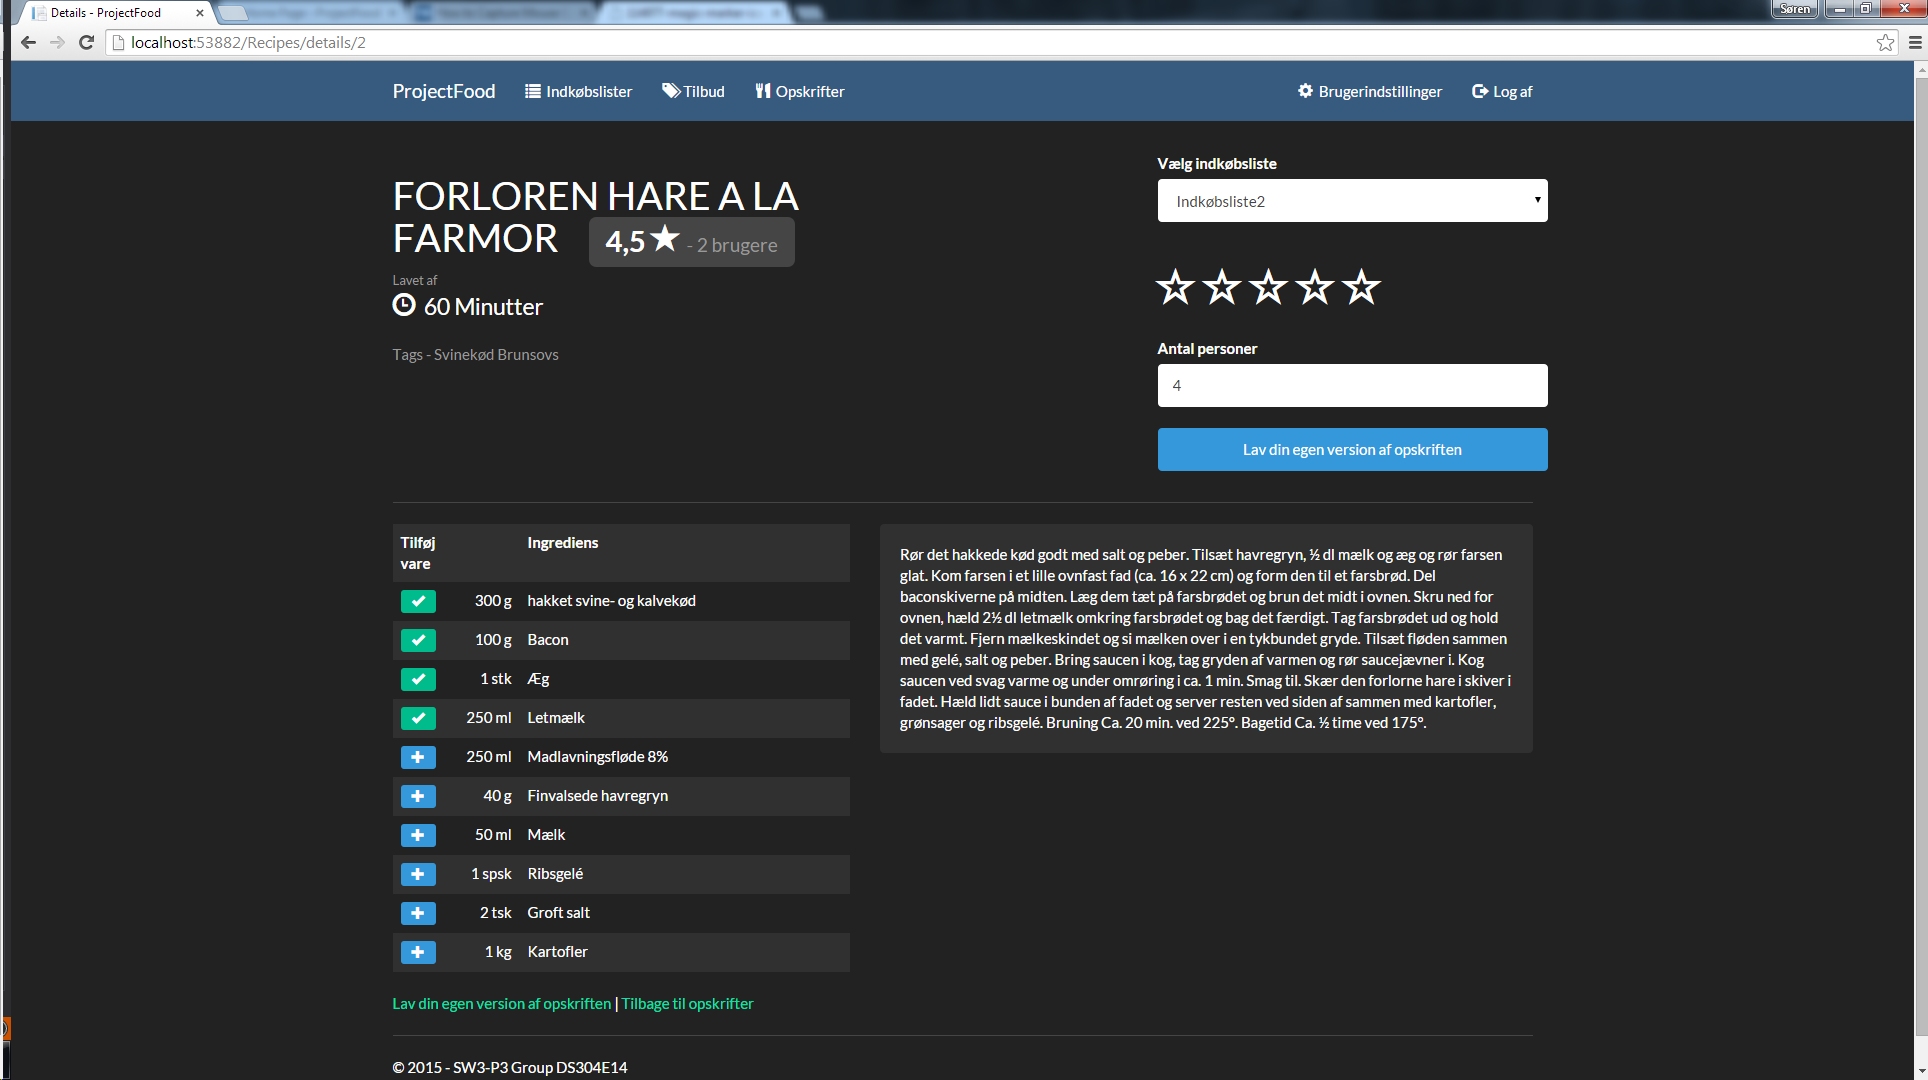
\includegraphics[width=1\textwidth,height=1\textheight,keepaspectratio, trim={1cm 0 0 16mm}, clip]{images/Screenshots/PickedRecipeOld.png}
	 
	 \vspace{2 mm}
	  
	  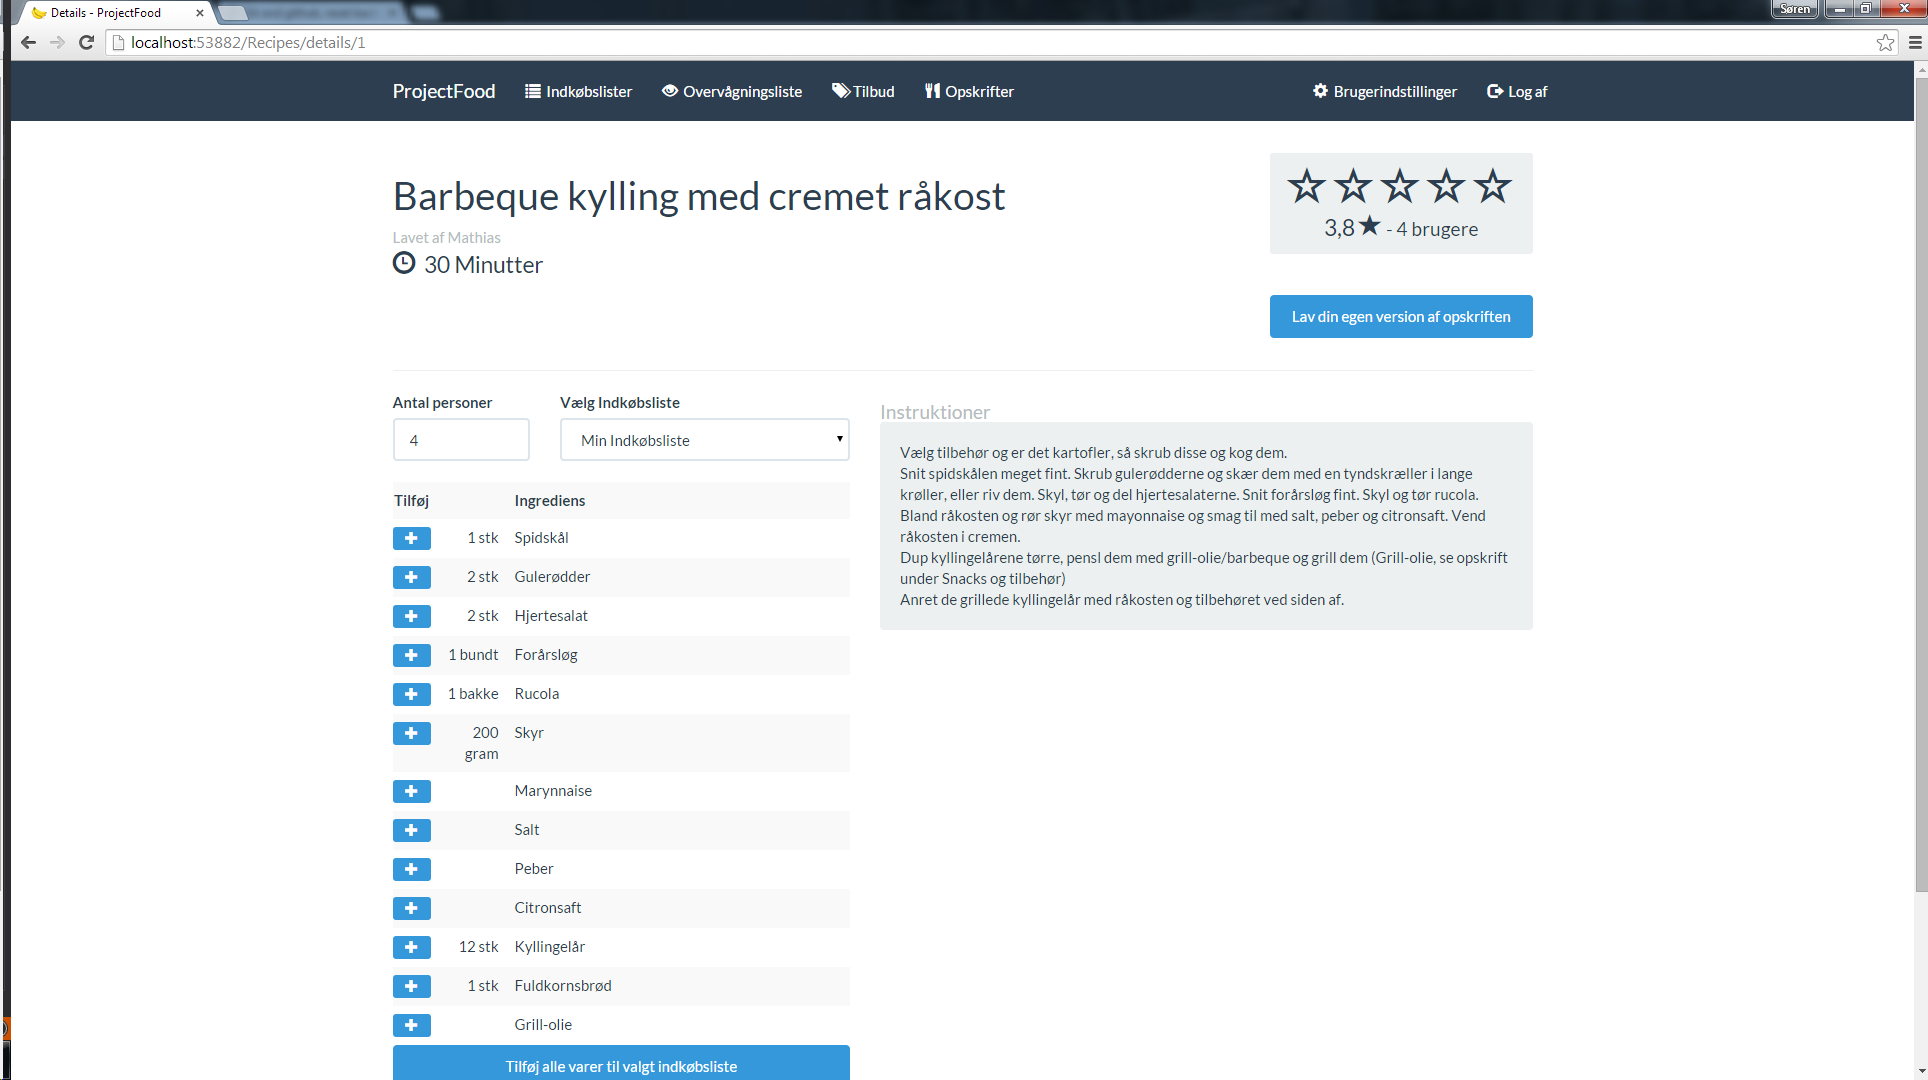
\includegraphics[width=1\textwidth,height=1\textheight,keepaspectratio, trim={1cm 0 0 16mm}, clip]{images/Screenshots/PickedRecipe.png}
	\end{column}
	\end{columns}
	

  \end{minipage}
  
  	
\end{frame}

\begin{frame}{Resultater}
\framesubtitle{Opskrifter}

	
	\begin{minipage}[0.3\textheight]{\textwidth}
	\begin{columns}[T]
	\begin{column}{1\textwidth}
	 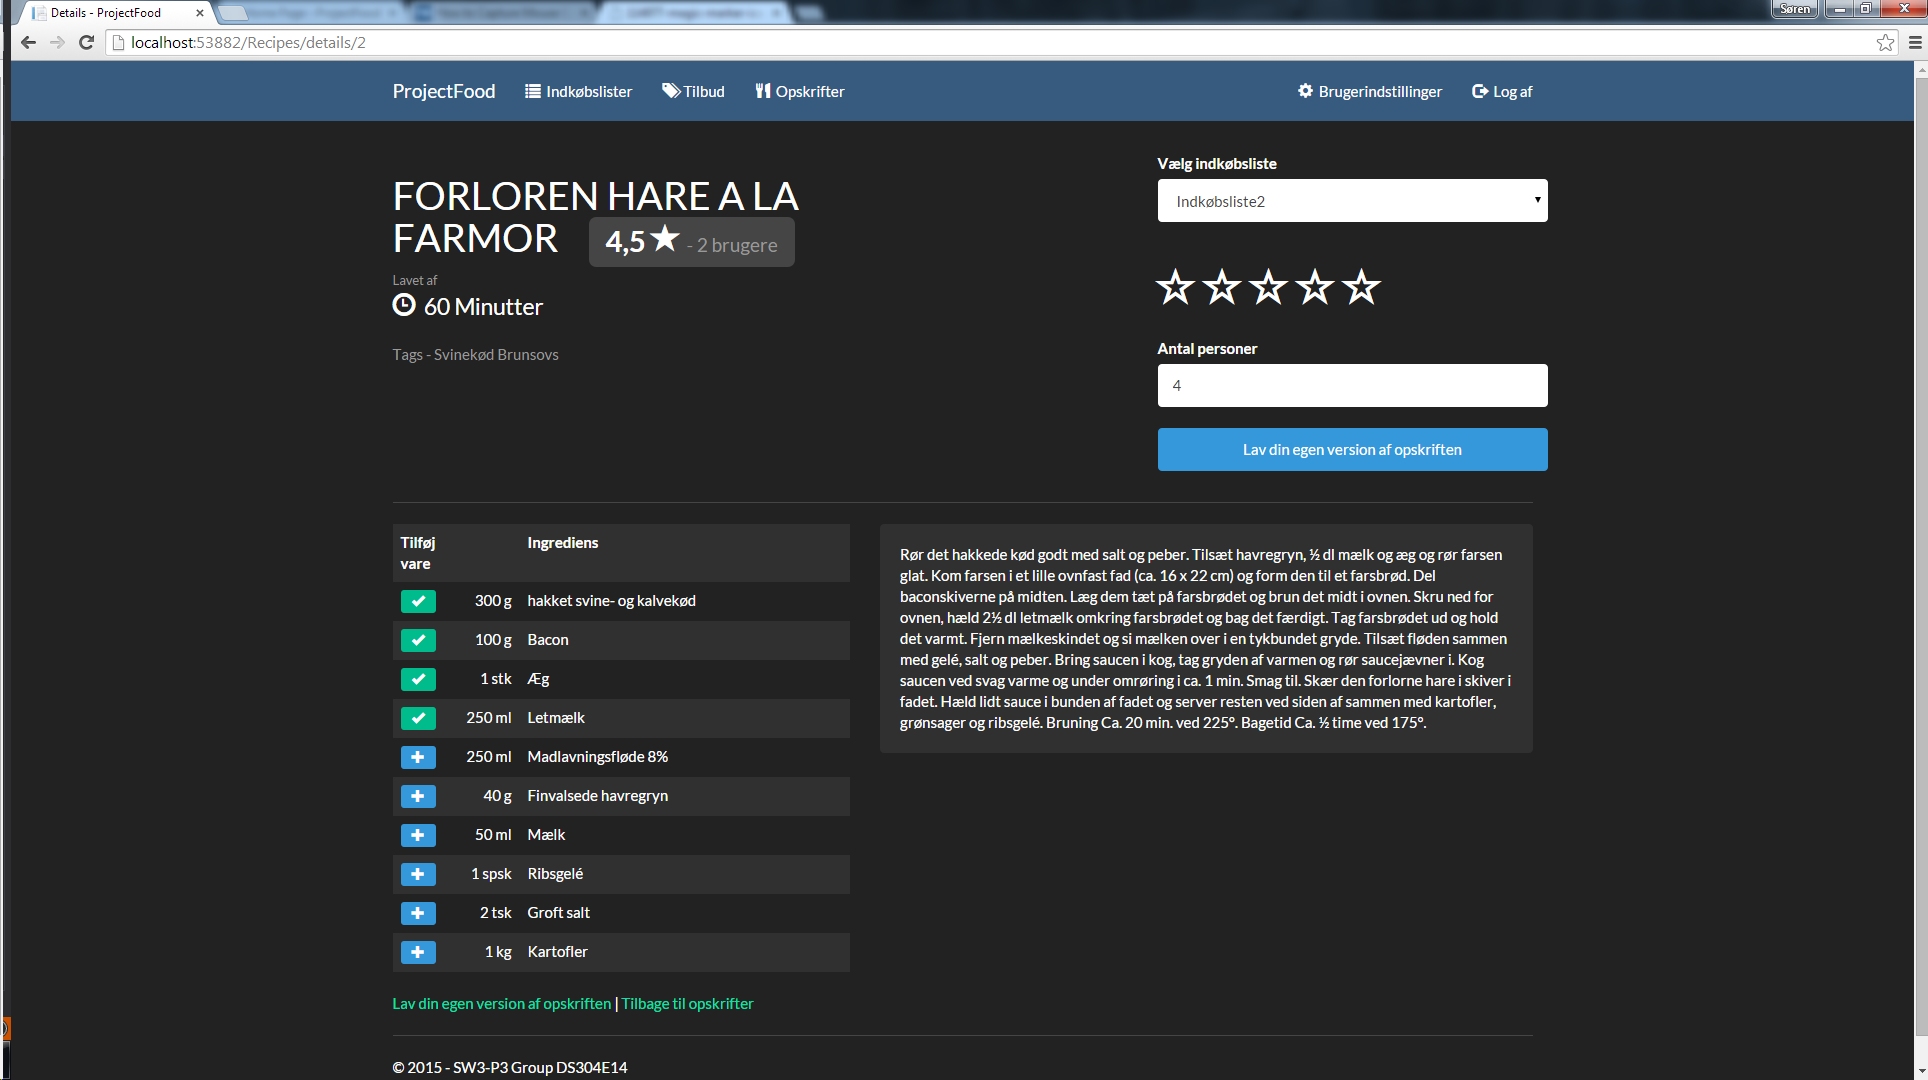
\includegraphics[width=1\textwidth,height=1\textheight,keepaspectratio, trim={1cm 0 0 16mm}, clip]{images/Screenshots/PickedRecipeOld.png}
	 
		\begin{itemize}
		\item Vælg indkøbsliste
		\item Funktion til at tilføje alle ingredienser.
		\item Kritisk, Kosmetisk
		\end{itemize}
	\end{column}

	\end{columns}

  \end{minipage}
	
\end{frame}
\begin{frame}{Resultater}
\framesubtitle{Opskrifter}

	
	\begin{minipage}[0.3\textheight]{\textwidth}
	\begin{columns}[T]
	\begin{column}{1\textwidth}
	 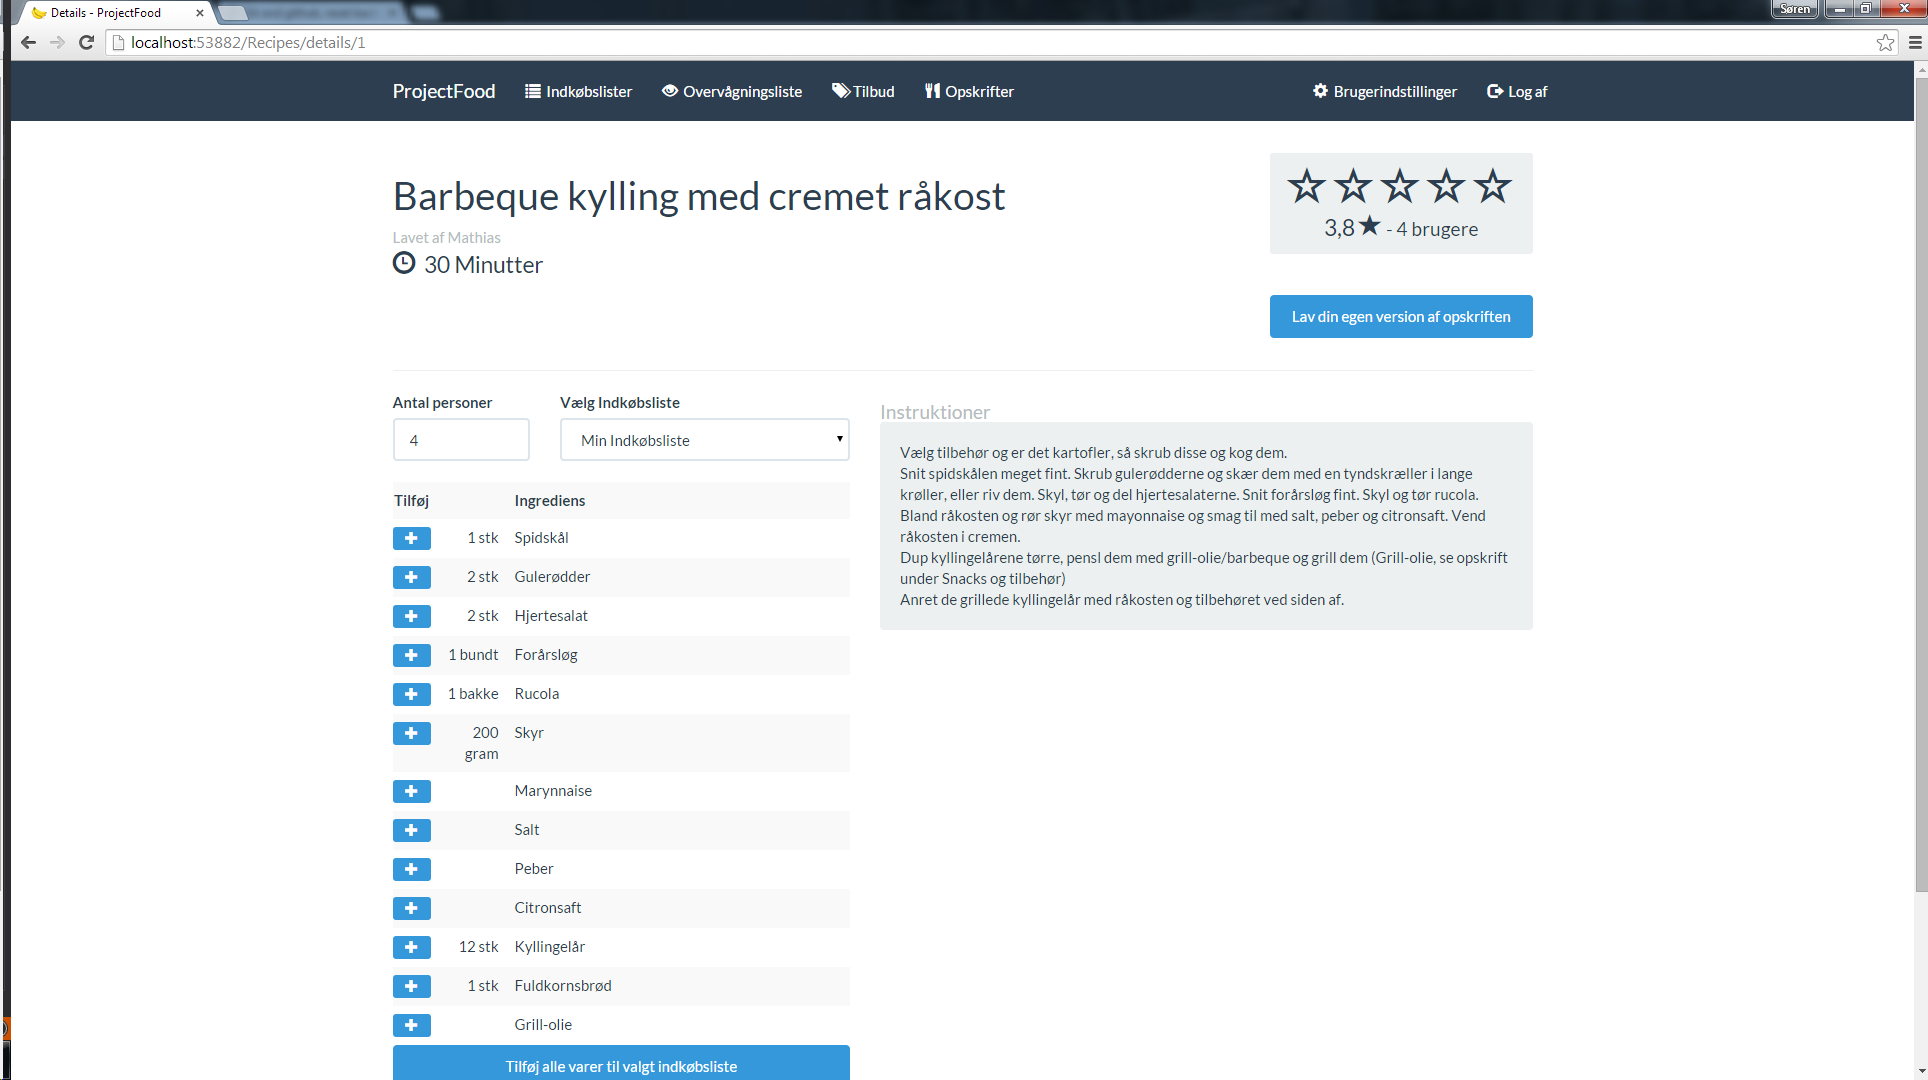
\includegraphics[width=1\textwidth,height=1\textheight,keepaspectratio, trim={1cm 0 0 16mm}, clip]{images/Screenshots/PickedRecipe.png}
	 
	 	\begin{itemize}
	 		\item Vælg indkøbsliste volder stadig problemer
	 		\item Kritisk
	 	\end{itemize}
	
	\end{column}

	\end{columns}

  \end{minipage}
	
\end{frame}

\begin{frame}{Konklusion på brugertests}
\subsection{Konklusion}
\framesubtitle{Hvad fik vi ud af det?}

	
\begin{itemize}
	\item Vi var ikke gode til at bruge vores design principper
		\begin{itemize}
			\item Proximity
			\item Feedback
			\item Navigation
			\item Consistency
		\end{itemize}
	\item Mange af problemerne blev udrettet i den endelige udgave
	\item Der var store problemer med Feedback, og Consistency
\end{itemize}
  
\end{frame}


\begin{frame}{Unit Tests}
\subsection{Unit Tests}
\framesubtitle{Hvorfor unit tests?}

\begin{itemize}
	\item Input $\rightarrow$ \texttt{SomeFunction} $\rightarrow$  Output
	\item Coverage
	\item Udbytte
	\begin{itemize}
		\item Fejlfinding
		\begin{itemize}
			\item \texttt{NullReferenceException} ved runtime
			\item Funktionsfejl
		\end{itemize}
		\item Forbedrer refactor mulighederne
	\end{itemize}
\end{itemize}

\end{frame}
\begin{frame}{Unit Tests}
\framesubtitle{Eksempel}
\hbox{\hspace{5 mm}\scalebox{0.8}{
	\lstinputlisting{code/test/Test.cs}  }} 

\end{frame}

\begin{frame}{Unit Tests}
\framesubtitle{Hvorfor unit tests?}

\begin{itemize}
	\item Input $\rightarrow$ \texttt{SomeFunction} $\rightarrow$  Output
	\item Coverage
	\item Udbytte
	\begin{itemize}
		\item Fejlfinding
				\begin{itemize}
					\item \texttt{NullReferenceException} ved runtime
					\item Funktionsfejl
				\end{itemize}
		\item Forbedrer refactor mulighederne
	\end{itemize}
\end{itemize}

\end{frame}
